\documentclass[conference]{IEEEtran}
\usepackage{graphicx}
\usepackage{booktabs}
\usepackage{amsmath}
\usepackage{array}
\usepackage{float}
\usepackage[hidelinks]{hyperref}

\title{How Do Hindi Speakers Search Their Mental Lexicons?\\\large Evidence From Verbal Fluency and Spatial Arrangement Tasks}
\author{BRSM Hindi Fluency Project}
\date{April 2026}

\begin{document}
\maketitle
\begin{abstract}
This paper studies how Hindi speakers retrieve words from memory. We analyze two tasks: Verbal Fluency Task (VFT) and Spatial Arrangement Method (SpAM). The dataset has 35 participants and 1040 responses. For primary statistical tests, we use only Hindi/Hinglish responses ($n=723$), and we keep English responses only for comparison context. We test domain-wise differences with Kruskal--Wallis tests, association patterns with Spearman correlation, and VFT sequence dynamics using within-cluster versus cluster-switch transitions. For cluster comparison, we use Adjusted Rand Index (ARI) and Normalized Mutual Information (NMI) between participant SpAM clusters and embedding-based semantic and phonetic clusters. Domain-level tests are mostly not statistically significant, but descriptive patterns are stable across tasks. We also build an equal-weight composite fluency score that combines VFT and SpAM features. The findings suggest that lexical search is structured, but the strength of structure is heterogeneous across participants and domains.
\end{abstract}

\section{Introduction}
The main research question is: \textit{How do Hindi speakers search their mental lexicons for information?}

Verbal fluency performance is often used to understand memory search and lexical organization. Recent work also shows that phonological information can support semantic retrieval \cite{Kumar2022}. At a broader lexical level, semantic similarity and word-form similarity can co-occur across languages \cite{Dautriche2016}. For spatial data collection of semantic structure, SpAM provides an efficient way to capture perceived similarity in two-dimensional layouts \cite{Hout2013}.

In this study, we combine VFT and SpAM. The motivation is simple: VFT gives retrieval dynamics (how many words, how fast), while SpAM gives organization dynamics (how words are grouped in space). Together, these two tasks can provide a richer view of lexical search.

\subsection{Research Questions}
To avoid repetition, the focused research questions are presented once in Table~\ref{tab:rq_simple}.

\begin{table*}[t]
\centering
\caption{Research questions and simple meaning}
\label{tab:rq_simple}
\footnotesize
\begin{tabular}{p{0.08\textwidth} p{0.52\textwidth} p{0.31\textwidth}}
\toprule
RQ & Formal research question & Simple meaning \\
\midrule
RQ1 & Do VFT productivity and retrieval speed differ across semantic domains? & Are some domains easier or faster for word retrieval? \\
RQ2 & Which participant-level variables are associated with VFT outcomes? & Which personal factors are related to better or worse VFT performance? \\
RQ3 & Does SpAM spatial compactness differ across domains? & Do some domains form tighter semantic maps in SpAM? \\
RQ4 & How strongly do participant SpAM clusters align with semantic and phonetic embedding-based clusters? & Do human clusters match model-based meaning/sound clusters? \\
RQ5 & Does a combined VFT+SpAM fluency score improve inference compared to VFT-only scoring? & Is combined scoring more informative than VFT-only scoring? \\
\bottomrule
\end{tabular}
\normalsize
\end{table*}

\subsection{Hypotheses}
We explicitly define null and alternative hypotheses for confirmatory analyses.

\begin{itemize}
  \item \textbf{H0$_1$:} Domain distributions of VFT word count are equal. \textbf{H1$_1$:} At least one domain differs.
  \item \textbf{H0$_2$:} Domain distributions of VFT mean retrieval time are equal. \textbf{H1$_2$:} At least one domain differs.
  \item \textbf{H0$_3$:} Domain distributions of SpAM compactness (mean nearest-neighbor distance) are equal. \textbf{H1$_3$:} At least one domain differs.
  \item \textbf{H0$_4$:} Positive ARI alignment occurs with probability $0.5$ (no directional tendency). \textbf{H1$_4$:} Positive ARI alignment occurs with probability $> 0.5$.
  \item \textbf{H0$_5$:} Domain distributions of VFT cluster-switch rate are equal. \textbf{H1$_5$:} At least one domain differs.
  \item \textbf{H0$_6$:} There is no monotonic association between VFT total output and Hindi confidence. \textbf{H1$_6$:} A monotonic association exists.
\end{itemize}

\section{Data and Task Design}
\subsection{Participants and Responses}
The processed dataset contains 35 sessions (one per participant) and 1040 rows. The domain labels are: \textit{animals}, \textit{body-parts}, \textit{colours}, and \textit{foods}. Language labels in the processed data are Hindi/Hinglish (723 rows) and English (317 rows).

Primary statistical analyses use only Hindi/Hinglish rows. English rows are not used for primary hypothesis testing.

\subsection{Two Tasks}
\textbf{VFT:} Participants produced as many words as possible within one minute for each category.

\textbf{SpAM:} Participants arranged generated words in 2D space using normalized $x,y$ coordinates based on perceived similarity.

\section{Methods}
\subsection{Feature Construction}
For each participant-domain unit, we computed:
\begin{itemize}
    \item \textbf{VFT features:} word count, lexical diversity, mean retrieval time.
  \item \textbf{VFT transition features:} within-cluster transitions and cluster-switch transitions over consecutive produced words.
    \item \textbf{SpAM features:} mean nearest-neighbor distance in $x,y$ space, participant cluster labels from hierarchical clustering, and agreement with semantic/phonetic cluster labels.
\end{itemize}

\subsection{Semantic and Phonetic Embedding Creation}
This part is important, so we describe it step by step.

\textbf{Step 1: Text normalization.}
Each word was converted to Unicode NFKC form, lowercased, and stripped of extra spaces.

\textbf{Step 2: Semantic embedding with a multilingual transformer.}
We generated dense sentence-level embeddings for normalized tokens using the Hugging Face Sentence-Transformers model \texttt{paraphrase-multilingual-MiniLM-L12-v2}. This model provides a shared multilingual semantic space suitable for short Hindi/Hinglish lexical items \cite{Reimers2019}.

\textbf{Step 3: Phonetic key generation.}
For each token, we generated a phonetic key using a deterministic Devanagari-to-Latin mapping. Then we removed vowels and collapsed repeated consonant symbols to reduce spelling noise and keep broad sound structure.

\textbf{Step 4: Phonetic embedding with the same transformer encoder.}
We encoded phonetic keys using the same multilingual transformer. This keeps the representation family consistent across semantic and phonetic channels while changing input form (surface word vs phonetic key).

\textbf{Step 5: Cluster generation and alignment.}
For each participant-domain unit:
\begin{itemize}
  \item SpAM clusters were built from $(x,y)$ coordinates using Ward hierarchical clustering.
  \item The number of clusters $k$ was selected by silhouette criterion over candidate values.
  \item Semantic and phonetic embeddings were clustered using K-means with the same $k$.
\end{itemize}

\textbf{Step 6: Similarity metrics.}
We compared cluster partitions using ARI \cite{Hubert1985} and NMI (normalized information overlap; \cite{Shannon1948}). Cluster-quality selection used silhouette-guided $k$ selection \cite{Rousseeuw1987}.

\subsection{Statistical Tests}
To stay aligned with BRSM methods and avoid assumption mismatch, test selection followed a normality-first rule:
\begin{itemize}
  \item For each domain-comparison endpoint, we first ran Shapiro--Wilk within each domain \cite{Shapiro1965}.
  \item If all groups were approximately normal ($p>0.05$), we used one-way ANOVA.
  \item If at least one group was non-normal, we used Kruskal--Wallis \cite{Kruskal1952}.
  \item For participant-level associations, we used Spearman rank correlation \cite{Spearman1904} because several involved variables were non-normal and relationships were treated as monotonic rather than strictly linear.
  \item For directional tendency of positive ARI values, we used a binomial sign test.
\end{itemize}

\begin{table*}[t]
\centering
\caption{Normality-first test decision framework used in this study}
\label{tab:test_decisions}
\footnotesize
\begin{tabular}{p{0.30\textwidth} p{0.23\textwidth} p{0.35\textwidth}}
\toprule
Analysis target & Decision rule & Test used in final analysis \\
\midrule
Domain-wise VFT word count & At least one domain failed Shapiro--Wilk & Kruskal--Wallis \\
Domain-wise VFT mean RT & At least one domain failed Shapiro--Wilk & Kruskal--Wallis \\
Domain-wise VFT cluster-switch rate & At least one domain failed Shapiro--Wilk & Kruskal--Wallis \\
Domain-wise SpAM compactness (mean NN distance) & At least one domain failed Shapiro--Wilk & Kruskal--Wallis \\
Participant-level outcome associations & Non-normality and monotonic relation target & Spearman correlation \\
ARI directional tendency & Sign direction over paired outcomes & Binomial sign test \\
\bottomrule
\end{tabular}
\normalsize
\end{table*}

\subsection{Composite Fluency Score}
We define a participant-domain score using standardized components:
\[
S_d = \frac{1}{6}\left(z_{\text{word}} + z_{\text{diversity}} + z_{\text{speed}} + z_{\text{spatial}} + z_{\text{semAlign}} + z_{\text{phoAlign}}\right)
\]
where all domains have equal weight. The participant score is:
\[
S_{\text{participant}} = \frac{1}{D}\sum_{d=1}^{D} S_d
\]
with $D$ equal to number of available domains for that participant.

\section{Results}
\subsection{Descriptive Patterns}
Table~\ref{tab:domain_summary} reports domain-level descriptive values for Hindi/Hinglish rows.

\begin{table*}[t]
\centering
\caption{Domain-level summary (Hindi/Hinglish subset)}
\label{tab:domain_summary}
\footnotesize
\begin{tabular}{lrrrr}
\toprule
Domain & Sess.-dom N & Mean words & Mean RT (ms) & Mean lex. div. \\
\midrule
colours & 4  & 10.25 & 5392.52 & 0.914 \\
animals & 28 & 8.321 & 7196.57 & 0.996 \\
body-parts & 23 & 8.304 & 7384.59 & 0.995 \\
foods & 35 & 7.371 & 6978.33 & 1.000 \\
\bottomrule
\end{tabular}
\normalsize
\end{table*}

\begin{figure}[t]
\centering
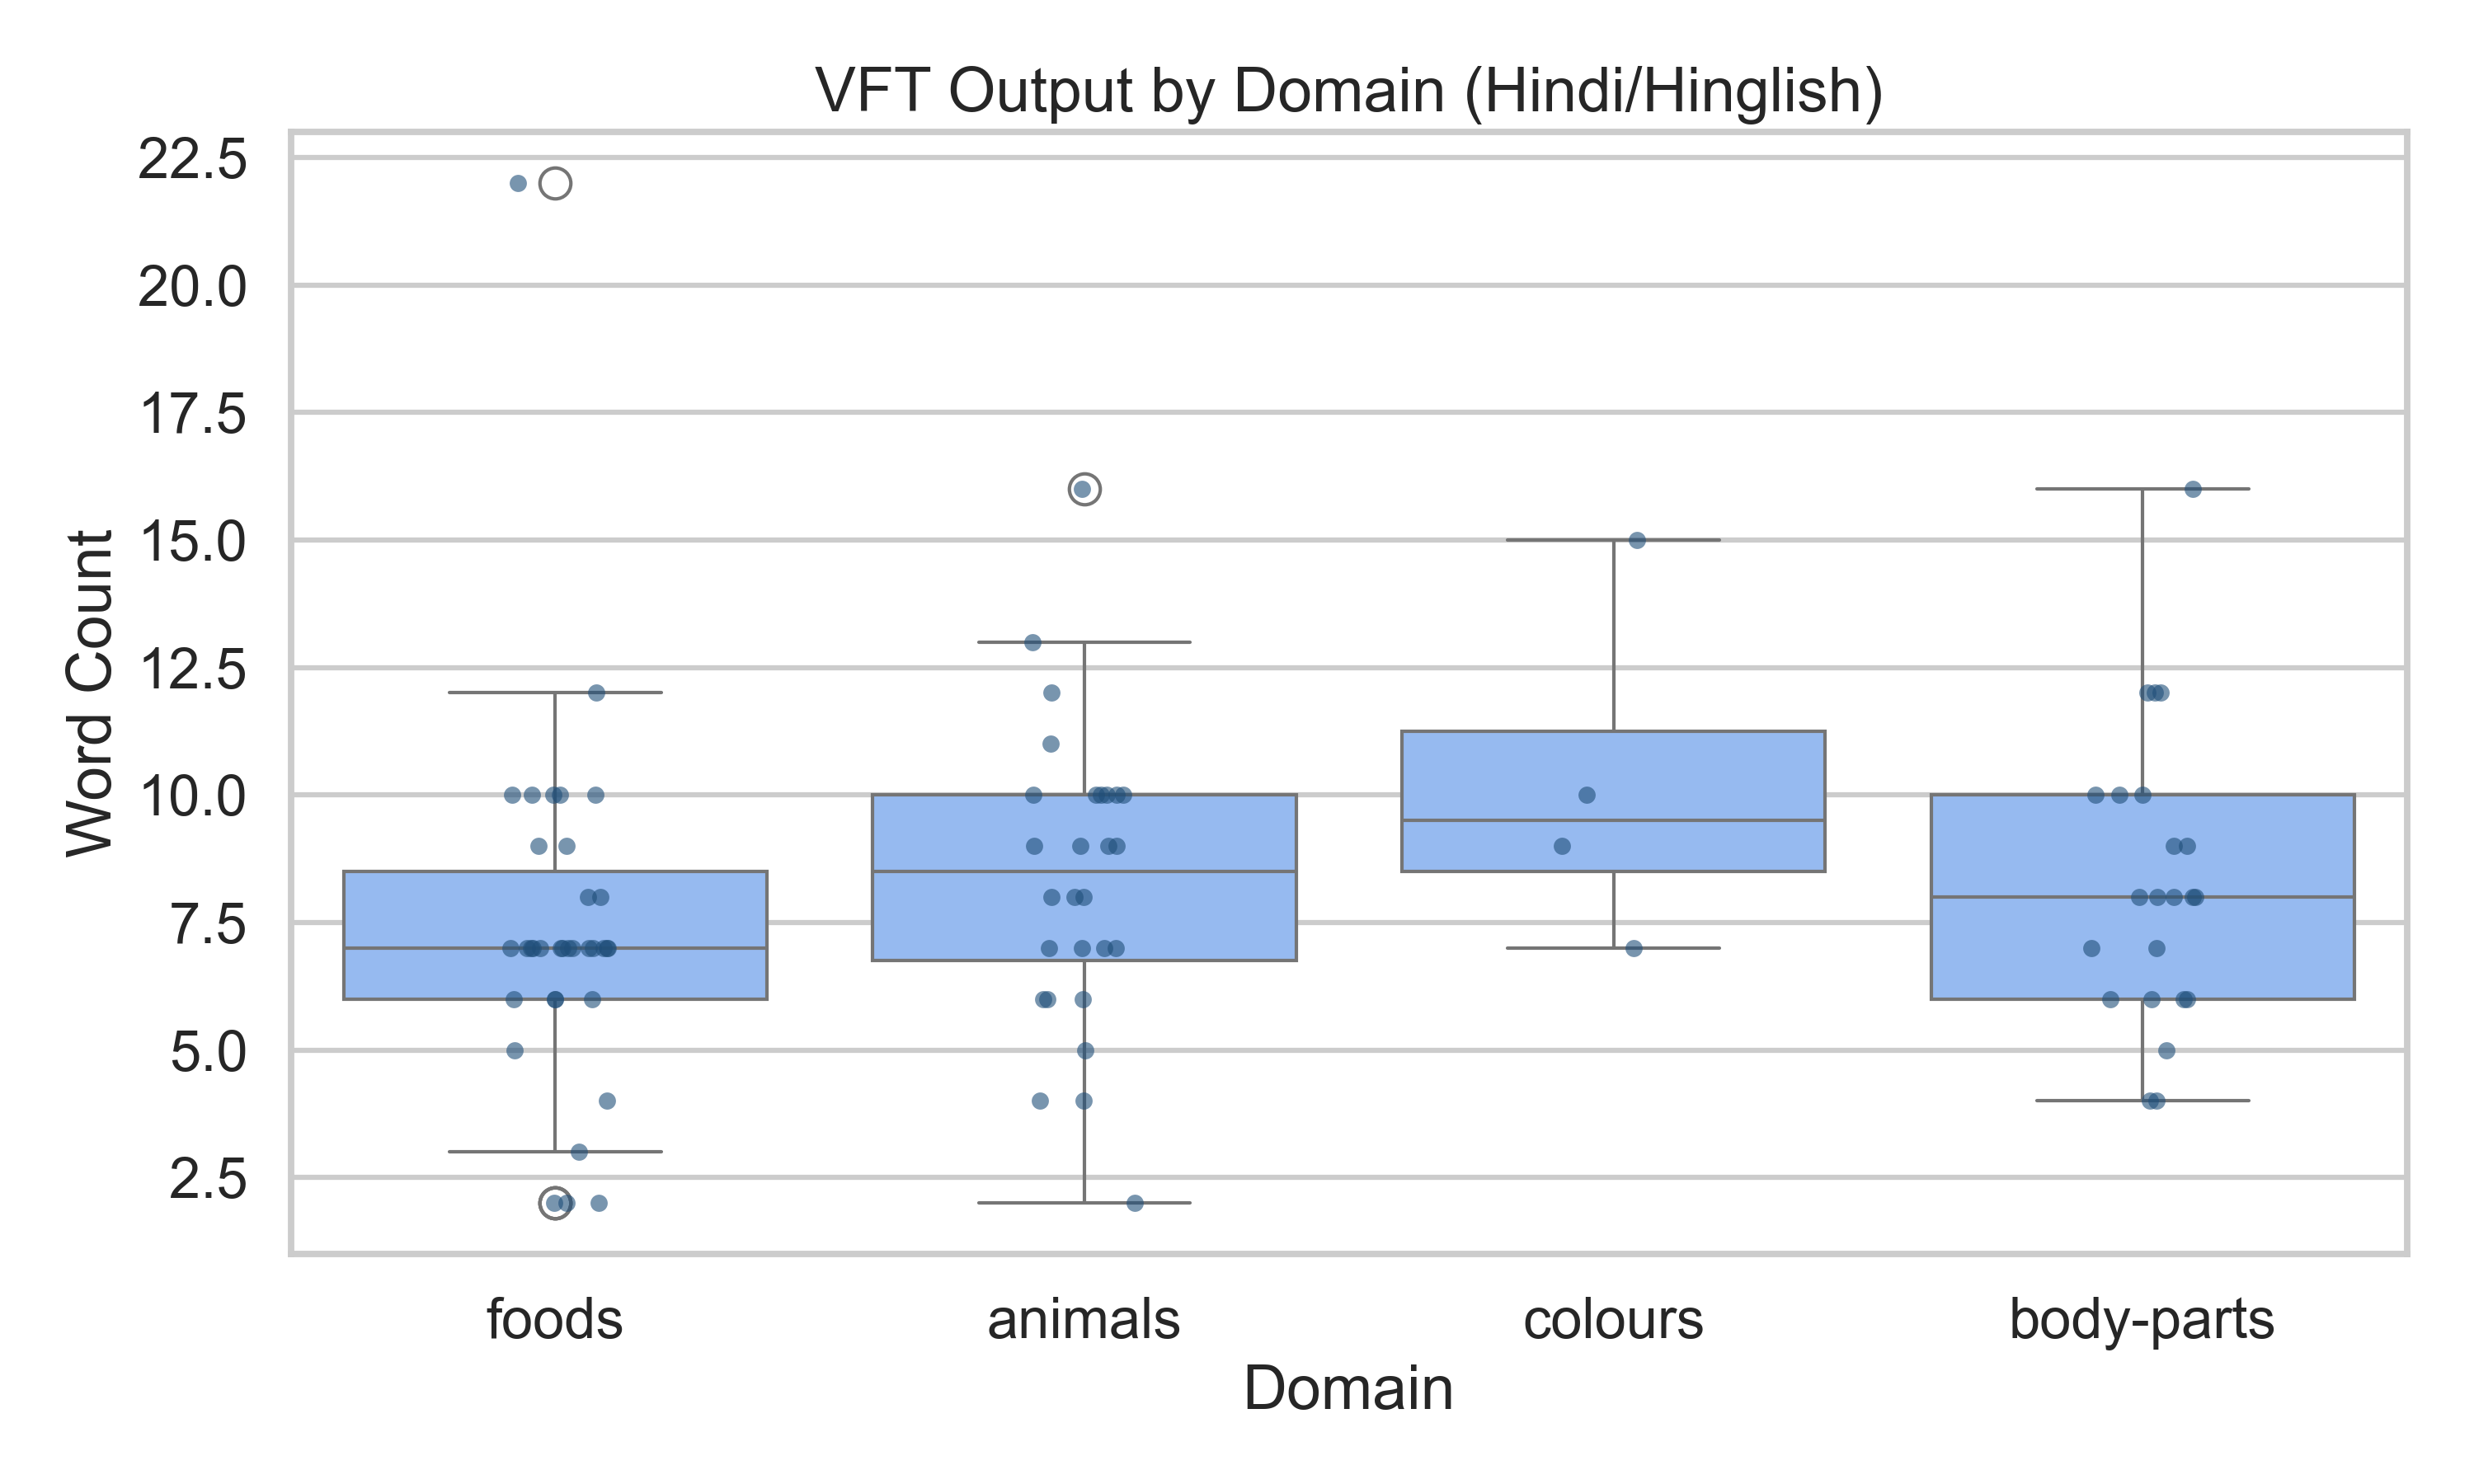
\includegraphics[width=\linewidth]{images/vft_wordcount_by_domain.png}
\caption{VFT word count by domain (Hindi/Hinglish subset).}
\label{fig:vft_count}
\end{figure}

\textbf{Interpretation.}
The descriptive view shows domain variability in output size, with colours having higher mean output in this sample. But this descriptive pattern still needs inferential testing.

\subsection{VFT Domain Tests}
\textbf{Question addressed (RQ1):} Do VFT productivity and retrieval speed differ across domains?

Based on the normality-first rule, Shapiro--Wilk indicated at least one non-normal domain distribution for both endpoints, so Kruskal--Wallis was applied.

\begin{itemize}
    \item Word count by domain: $H=5.295$, $p=0.1515$ (not significant).
    \item Mean RT by domain: $H=1.919$, $p=0.5894$ (not significant).
\end{itemize}

\begin{figure}[t]
\centering
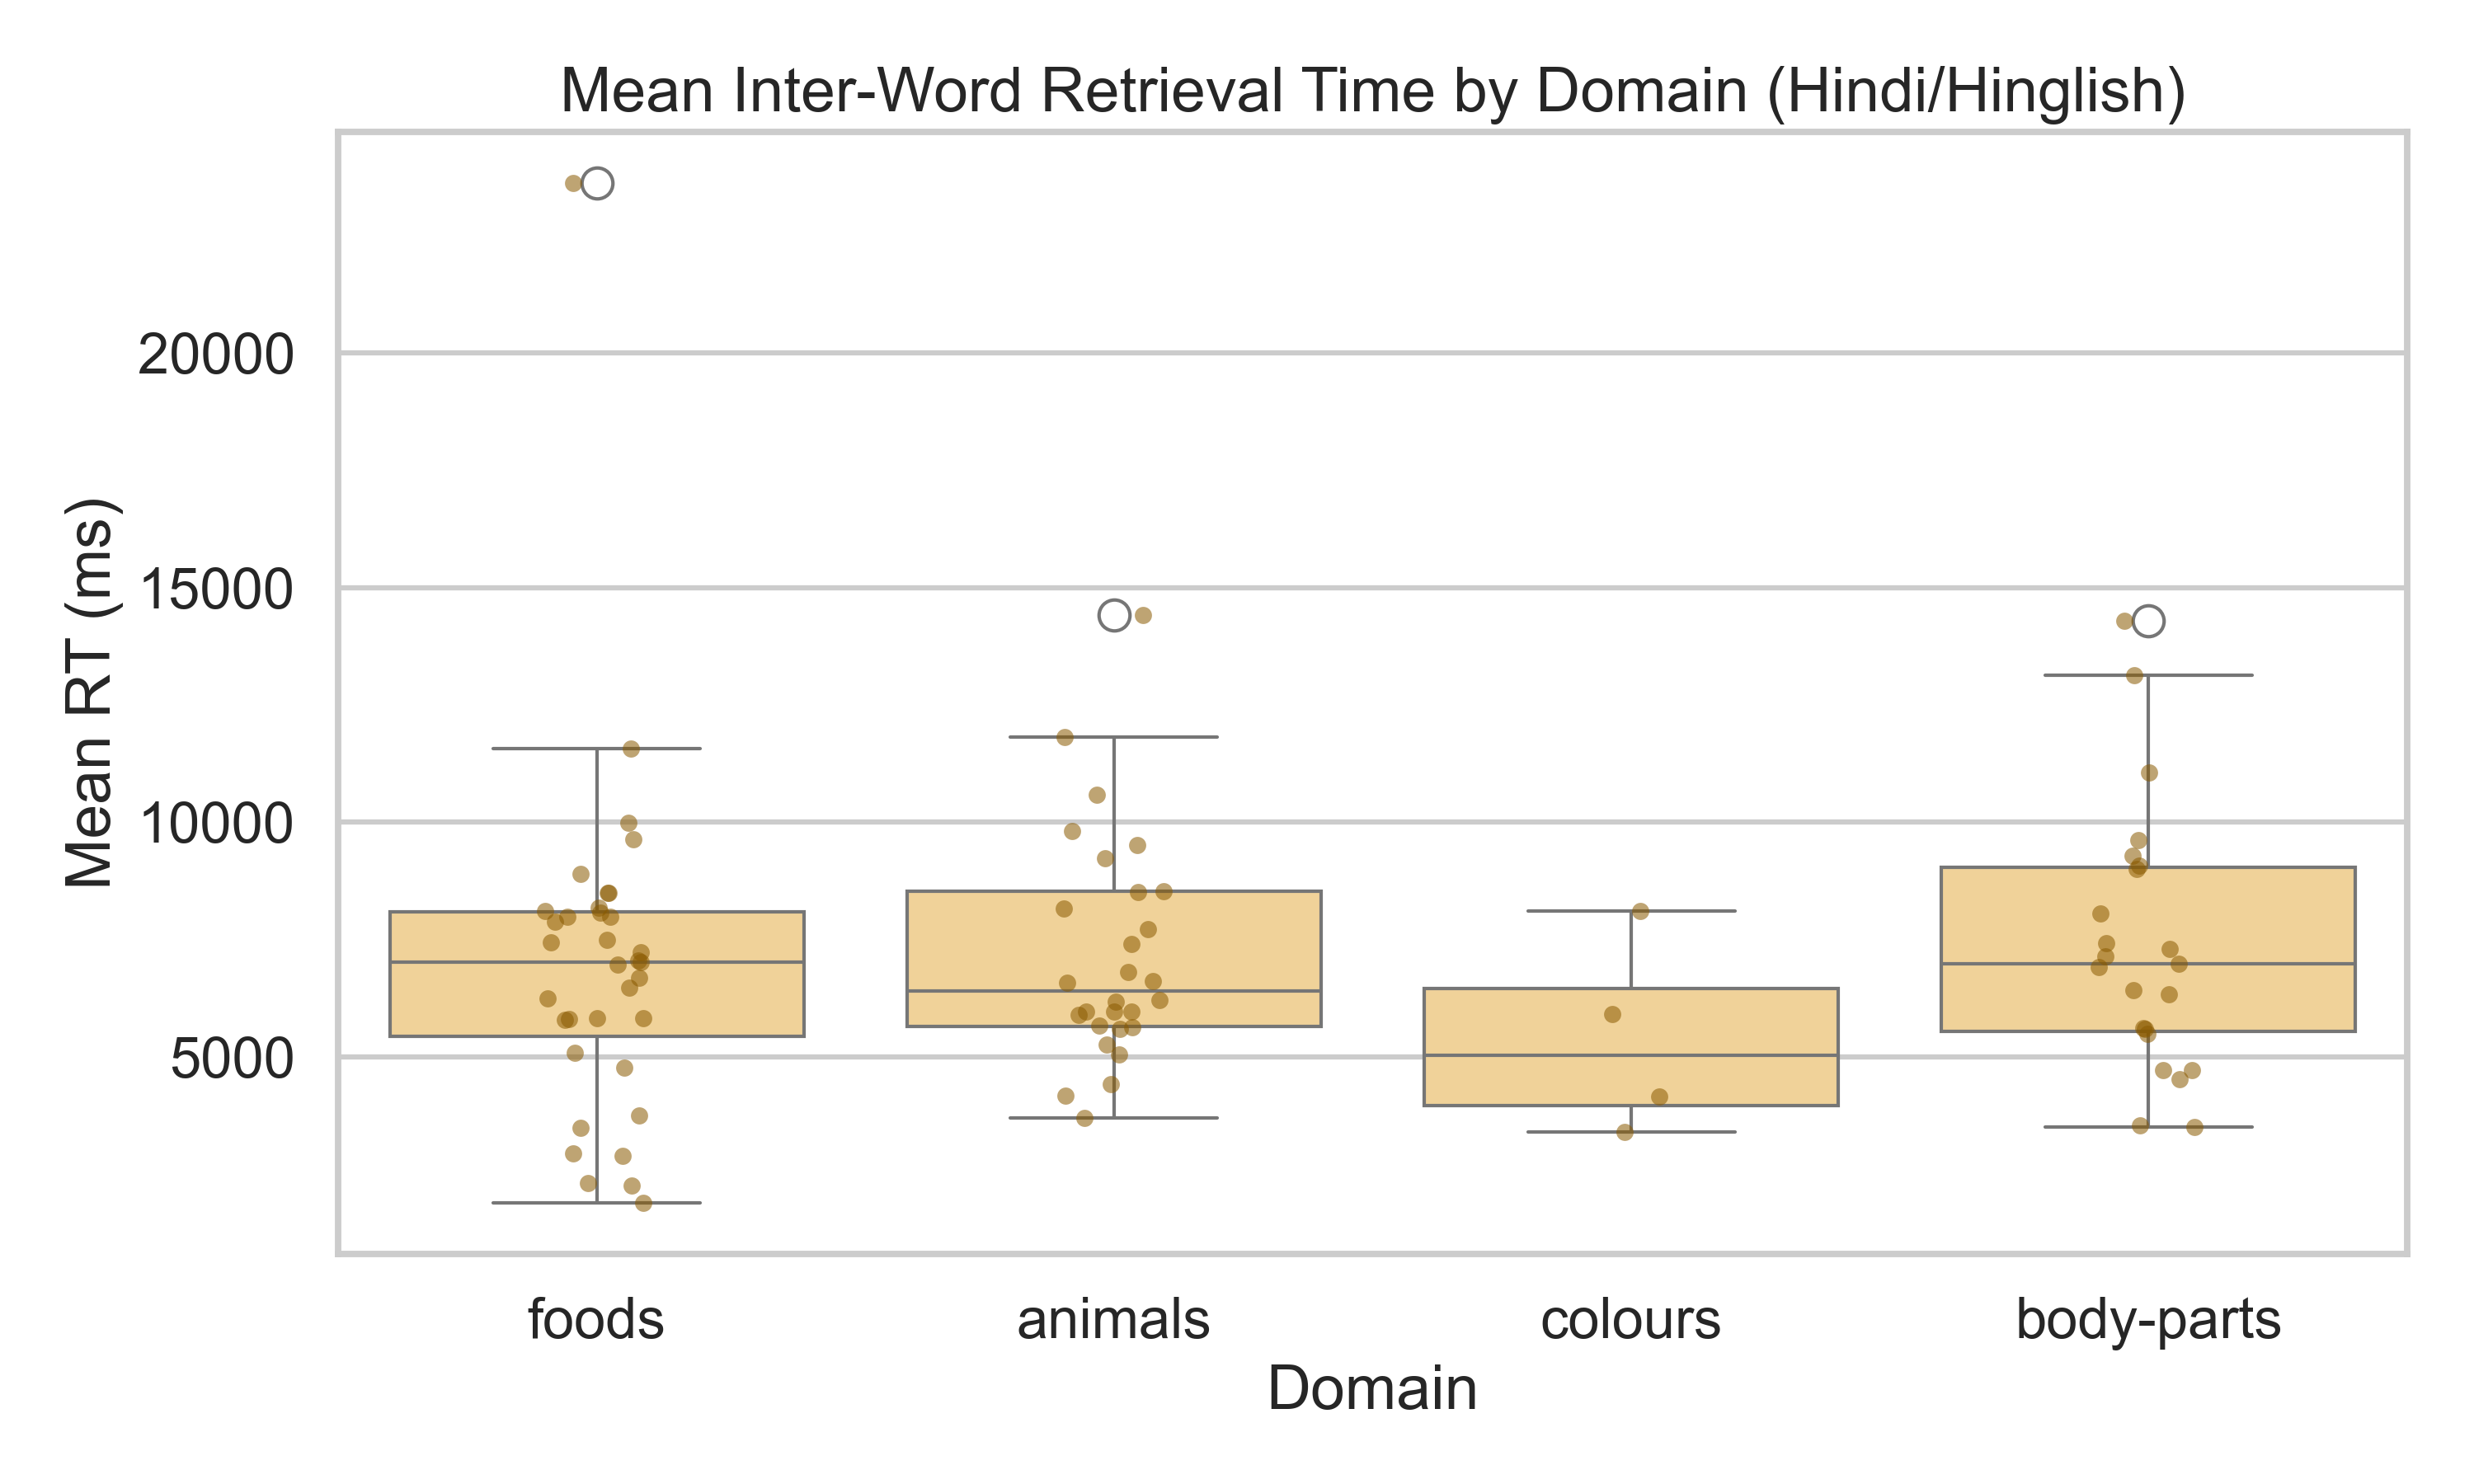
\includegraphics[width=\linewidth]{images/vft_rt_by_domain.png}
\caption{Mean retrieval time by domain (Hindi/Hinglish subset).}
\label{fig:vft_rt}
\end{figure}

\begin{figure}[t]
\centering
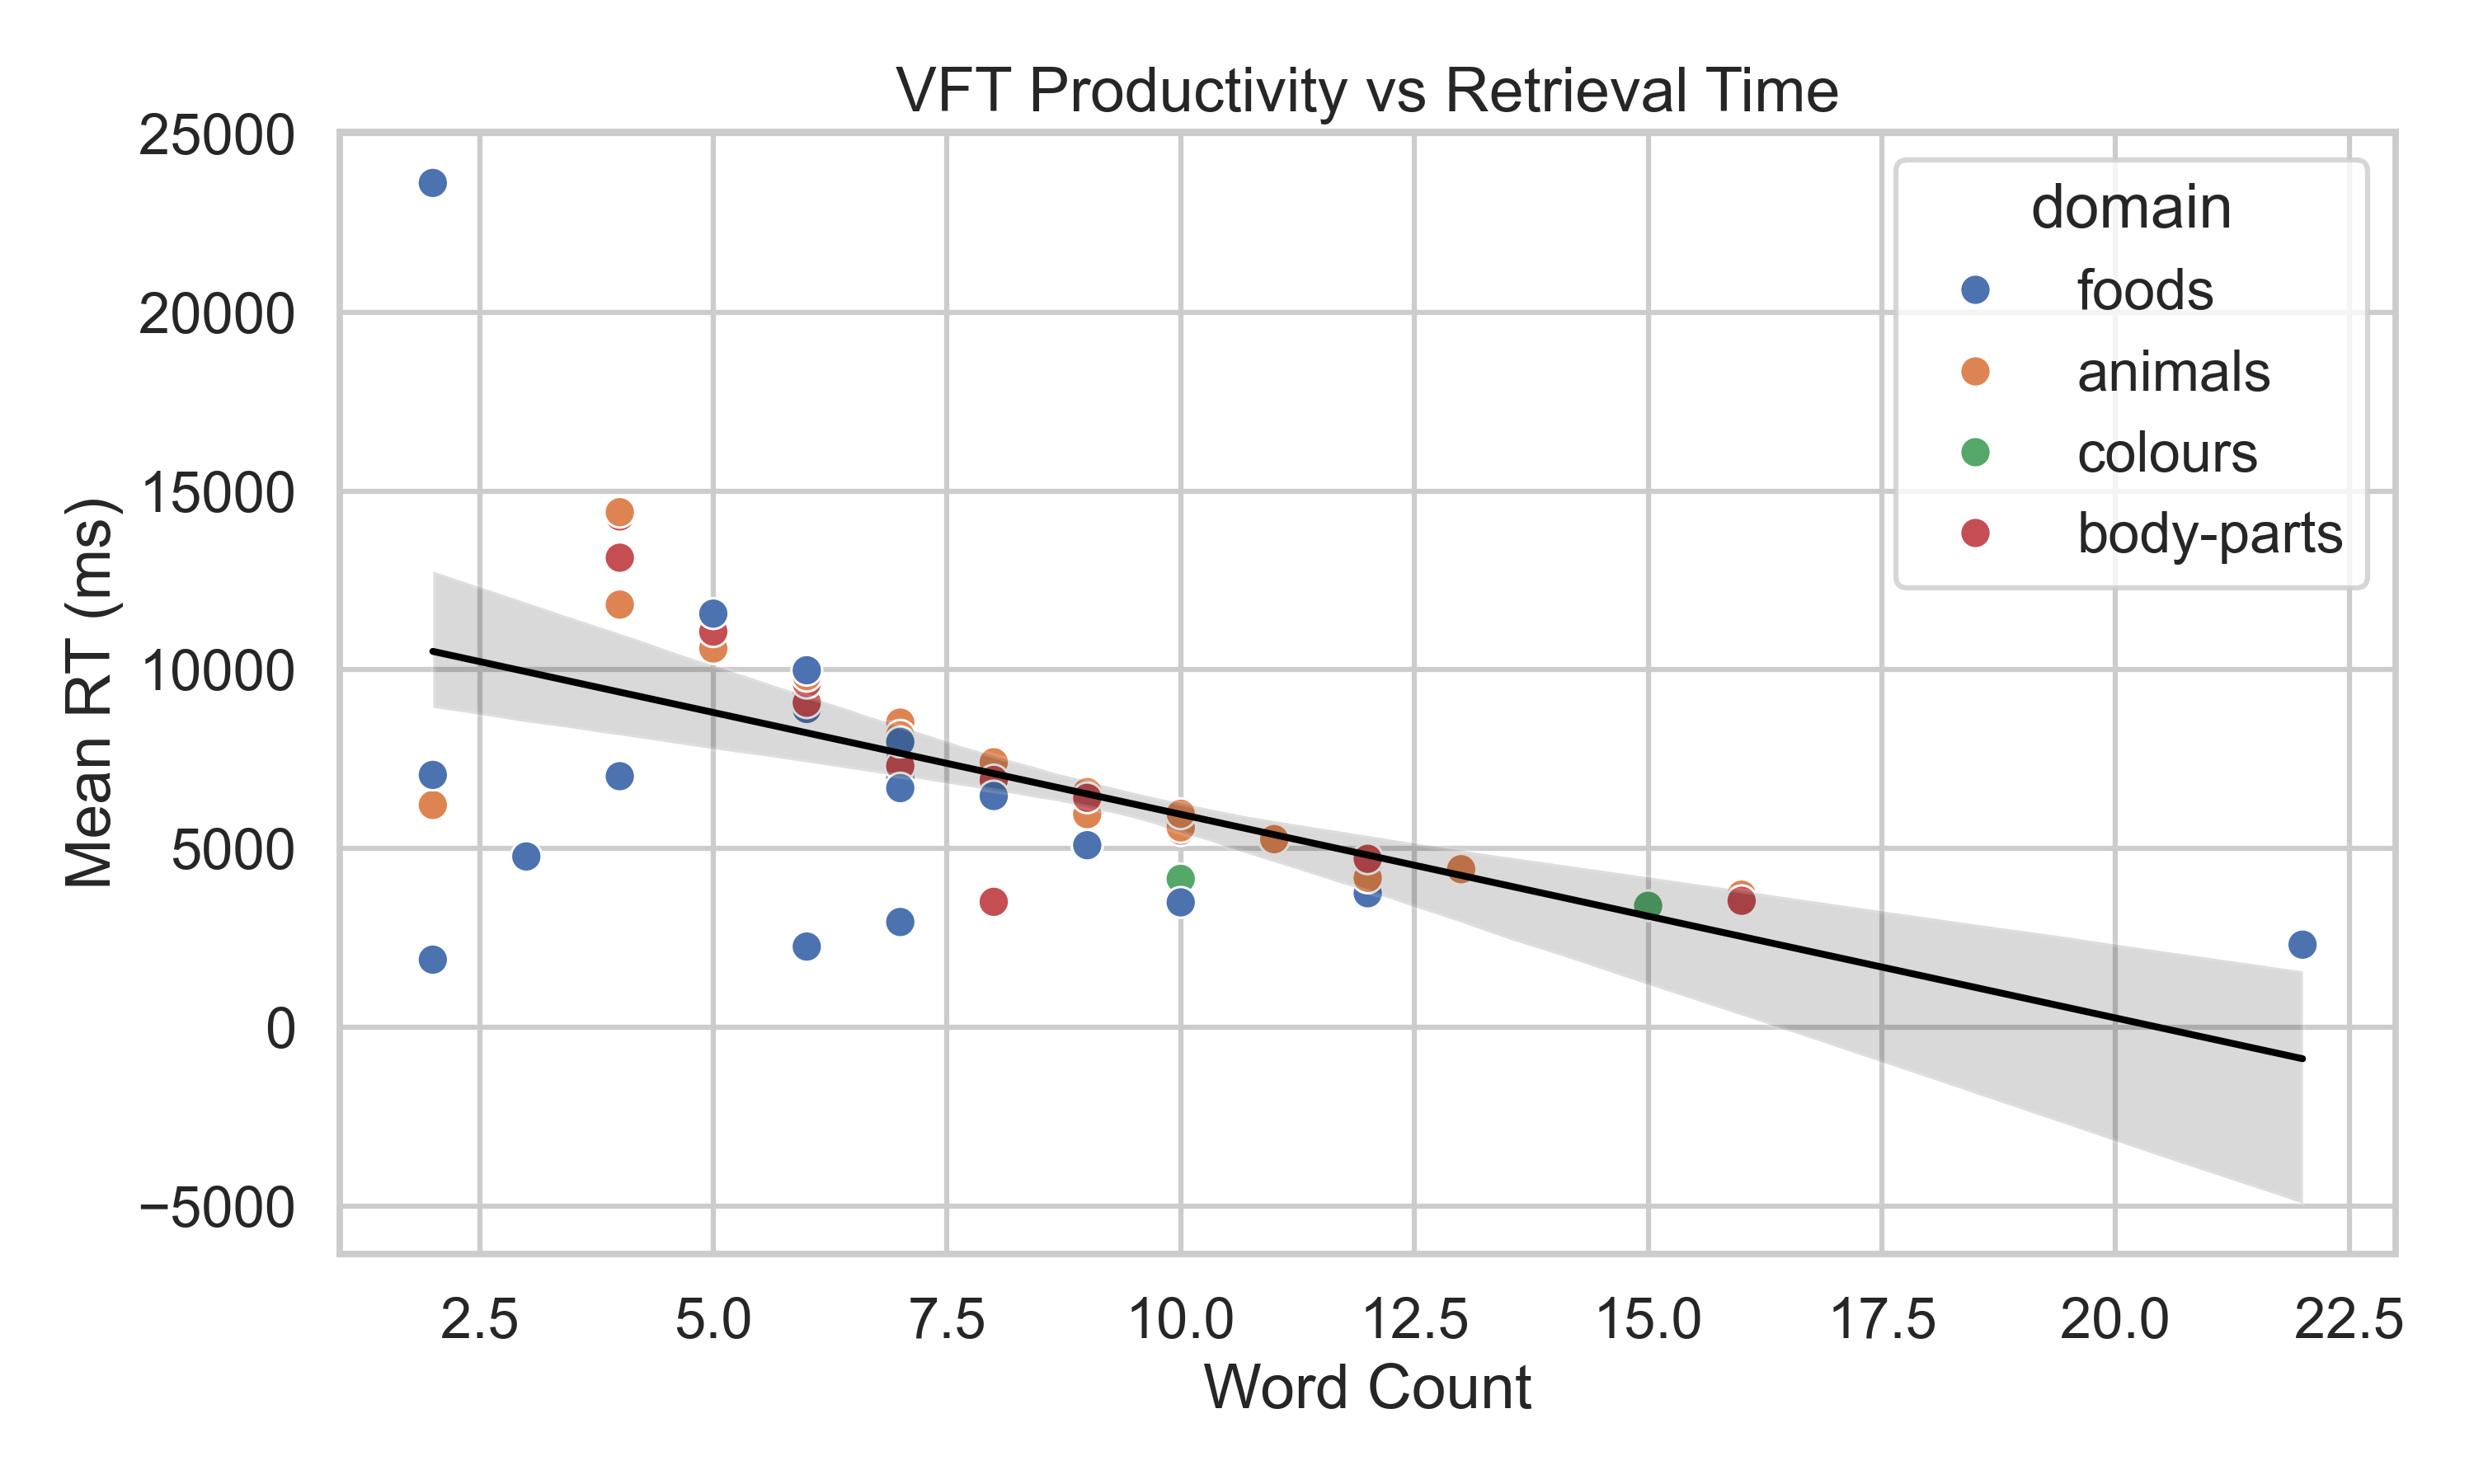
\includegraphics[width=\linewidth]{images/vft_words_vs_rt.png}
\caption{Relation between VFT output size and retrieval speed.}
\label{fig:vft_scatter}
\end{figure}

\textbf{Inference.}
For RQ1, we do not reject the null hypothesis at $\alpha=0.05$. Domain differences are present descriptively, but inferential evidence is not strong in this sample.

\subsection{VFT Transition Dynamics (Within-Cluster vs Cluster-Switch)}
This subsection addresses the missing process-level part of VFT analysis by examining how participants moved through clusters over time.

For each participant-domain sequence, words were ordered by production position. Using participant SpAM-derived clusters in that domain, each adjacent word pair $(w_t, w_{t+1})$ was labeled as:
\begin{itemize}
  \item \textbf{within-cluster transition} if both words had the same cluster label,
  \item \textbf{cluster-switch transition} if labels differed.
\end{itemize}

\begin{table*}[t]
\centering
\caption{VFT transition summary by domain}
\label{tab:vft_transition_summary}
\scriptsize
\begin{tabular}{@{}lrrrrrr@{}}
\toprule
Domain & N & Mean words & Mean within & Mean switch & Within rate & Switch rate \\
\midrule
colours & 4  & 10.250 & 4.500 & 4.750 & 0.456 & 0.544 \\
animals & 27 & 8.556  & 4.037 & 3.519 & 0.532 & 0.468 \\
foods & 31 & 8.032 & 3.871 & 3.161 & 0.537 & 0.463 \\
body-parts & 23 & 8.304 & 4.391 & 2.913 & 0.591 & 0.409 \\
\bottomrule
\end{tabular}
\normalsize
\end{table*}

Domain differences in switch-rate were tested with Kruskal--Wallis (normality-first rule): $H=1.909$, $p=0.5916$.

Exploratory session-level associations were also weak and non-significant:
\begin{itemize}
  \item total words vs switch-rate: $\rho=-0.043$, $p=0.8147$;
  \item Hindi confidence vs switch-rate: $\rho=0.180$, $p=0.3230$.
\end{itemize}

\textbf{Inference.}
Within-cluster and cluster-switch transitions are now explicitly quantified, but in this sample they do not show strong domain effects or strong association with confidence. Thus, transition behavior should be interpreted as descriptive support for strategy heterogeneity, not as a confirmed group-level effect.

\subsection{Associations With Background Variables}
\textbf{Question addressed (RQ2):} Which participant-level variables are associated with VFT outcomes?

Spearman correlation was selected because normality assumptions were not consistently satisfied and the target relation was monotonic.

At session level, significant Spearman results include:
\begin{itemize}
    \item Total words vs Hindi confidence: $\rho=-0.395$, $p=0.019$.
\end{itemize}

\textbf{Interpretation.}
This indicates a moderate negative monotonic relationship: participants with higher total VFT output tended to report lower Hindi confidence in this sample.

The direction is counter-intuitive and should not be over-interpreted. A plausible explanation is measurement mismatch: confidence is self-reported and can reflect perceived ability rather than objective lexical performance. More fluent participants may under-rate themselves, while less fluent participants may over-rate themselves. Another possibility is strategy variation: some lower-confidence participants may produce more words through risk-taking, whereas highly confident participants may answer more cautiously. Finally, the modest sample size ($n=35$) increases sensitivity to outliers and sampling variation.

\textbf{Inference.}
For RQ2, there is evidence of a statistically significant participant-level association, but the negative direction is not theoretically straightforward and is likely influenced by self-report bias, strategy differences, and sample-size limitations.

\subsection{SpAM Domain Test}
\textbf{Question addressed (RQ3):} Does SpAM spatial compactness differ across domains?

Shapiro--Wilk diagnostics indicated at least one non-normal domain distribution for compactness, so Kruskal--Wallis was used.

Mean nearest-neighbor distance by domain gave $H=3.038$, $p=0.3857$ (not significant).

\begin{figure}[t]
\centering
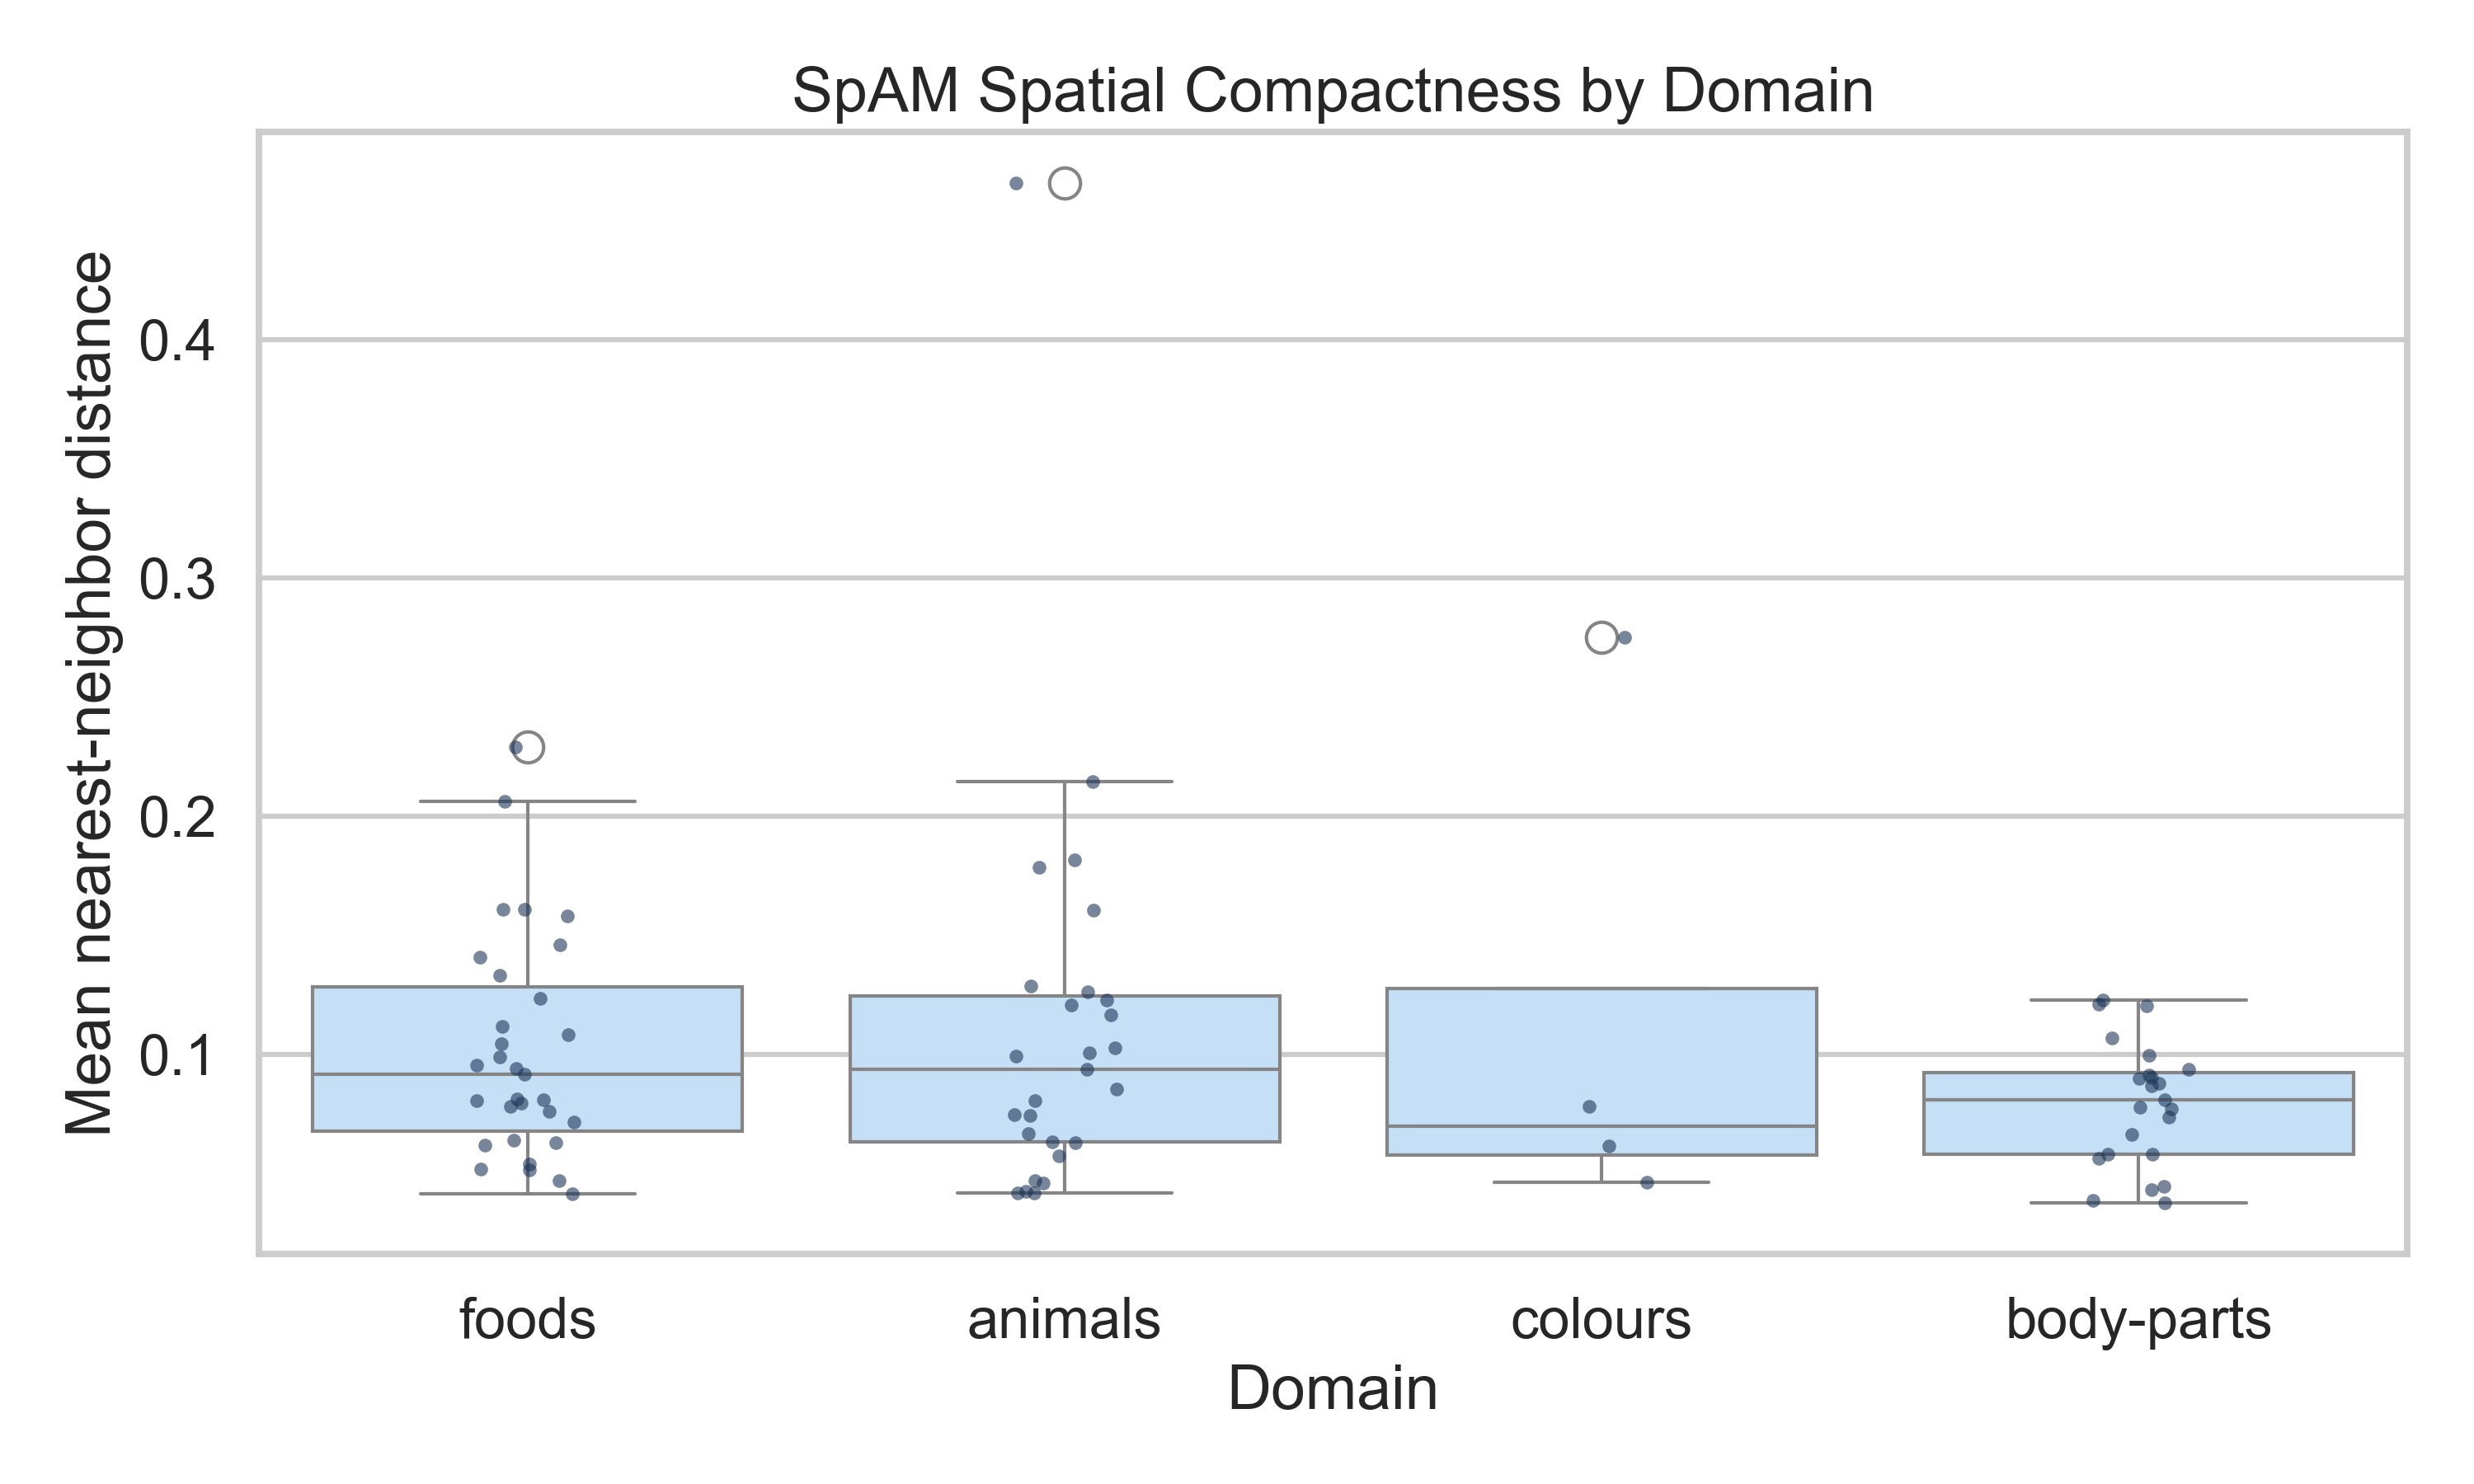
\includegraphics[width=\linewidth]{images/spam_compactness_by_domain.png}
\caption{SpAM compactness (mean nearest-neighbor distance) by domain.}
\label{fig:spam_compactness}
\end{figure}

\textbf{Inference.}
For RQ3, domain-wise compactness differences are not statistically significant, so we treat them as descriptive only.

\subsection{Cluster Similarity Metrics}
\textbf{Question addressed (RQ4):} How strongly do participant SpAM clusters align with semantic and phonetic embedding-based clusters?

Table~\ref{tab:cluster_summary} shows domain-wise mean agreement values.

\begin{table*}[t]
\centering
\caption{Domain-wise mean cluster similarity metrics}
\label{tab:cluster_summary}
\footnotesize
\begin{tabular}{lrrrrr}
\toprule
Domain & ARI(sem,SpAM) & ARI(pho,SpAM) & NMI(sem,SpAM) & NMI(pho,SpAM) & Mean NN distance \\
\midrule
foods & 0.086 & 0.106 & 0.364 & 0.370 & 0.102 \\
body-parts & 0.316 & 0.162 & 0.490 & 0.340 & 0.079 \\
colours & 0.157 & 0.175 & 0.301 & 0.319 & 0.115 \\
animals & 0.095 & 0.064 & 0.394 & 0.384 & 0.111 \\
\bottomrule
\end{tabular}
\normalsize
\end{table*}

Global means were: ARI(sem,SpAM)=0.154, ARI(pho,SpAM)=0.111, NMI(sem,SpAM)=0.405, NMI(pho,SpAM)=0.364.

Sign tests for positive ARI tendency were significant:
\begin{itemize}
  \item semantic-SpAM ARI: 48/78 positive, $p=0.0268$.
  \item phonetic-SpAM ARI: 48/79 positive, $p=0.0356$.
\end{itemize}

  \begin{figure}[t]
  \centering
  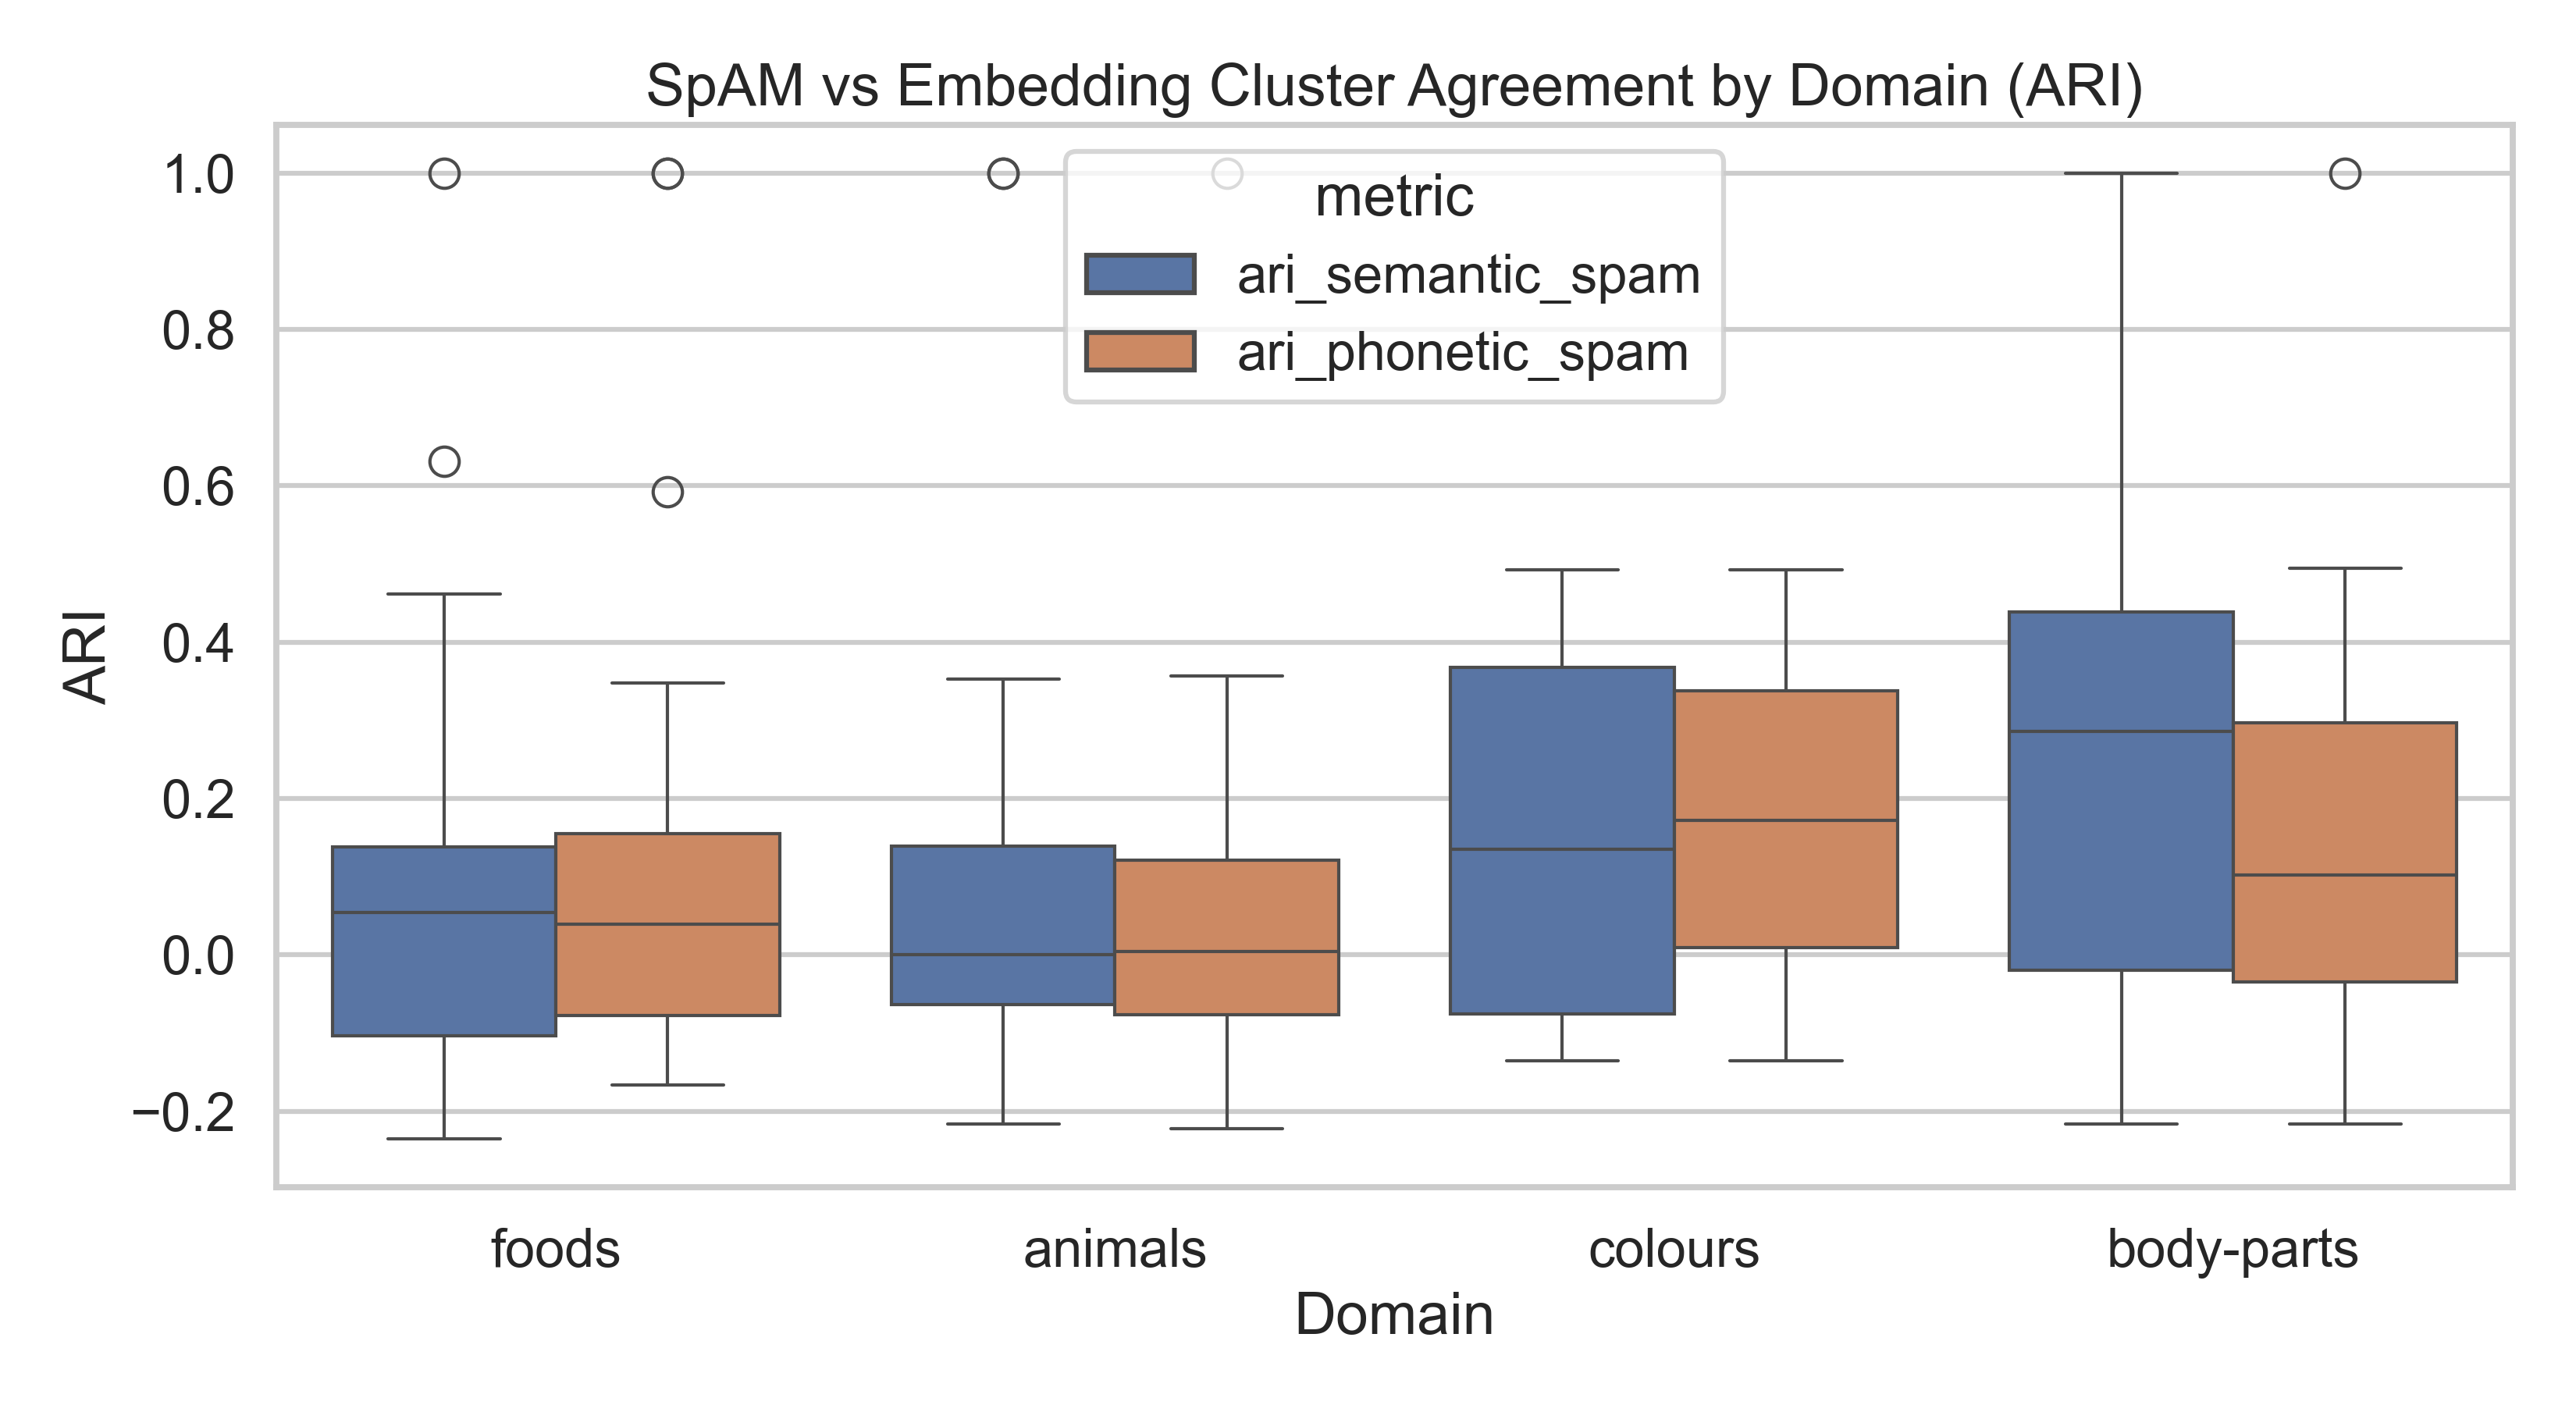
\includegraphics[width=\linewidth]{images/spam_alignment_by_domain.png}
  \caption{Domain-wise ARI alignment between participant SpAM clusters and embedding-based clusters.}
  \label{fig:spam_ari}
  \end{figure}

  \begin{figure}[t]
  \centering
  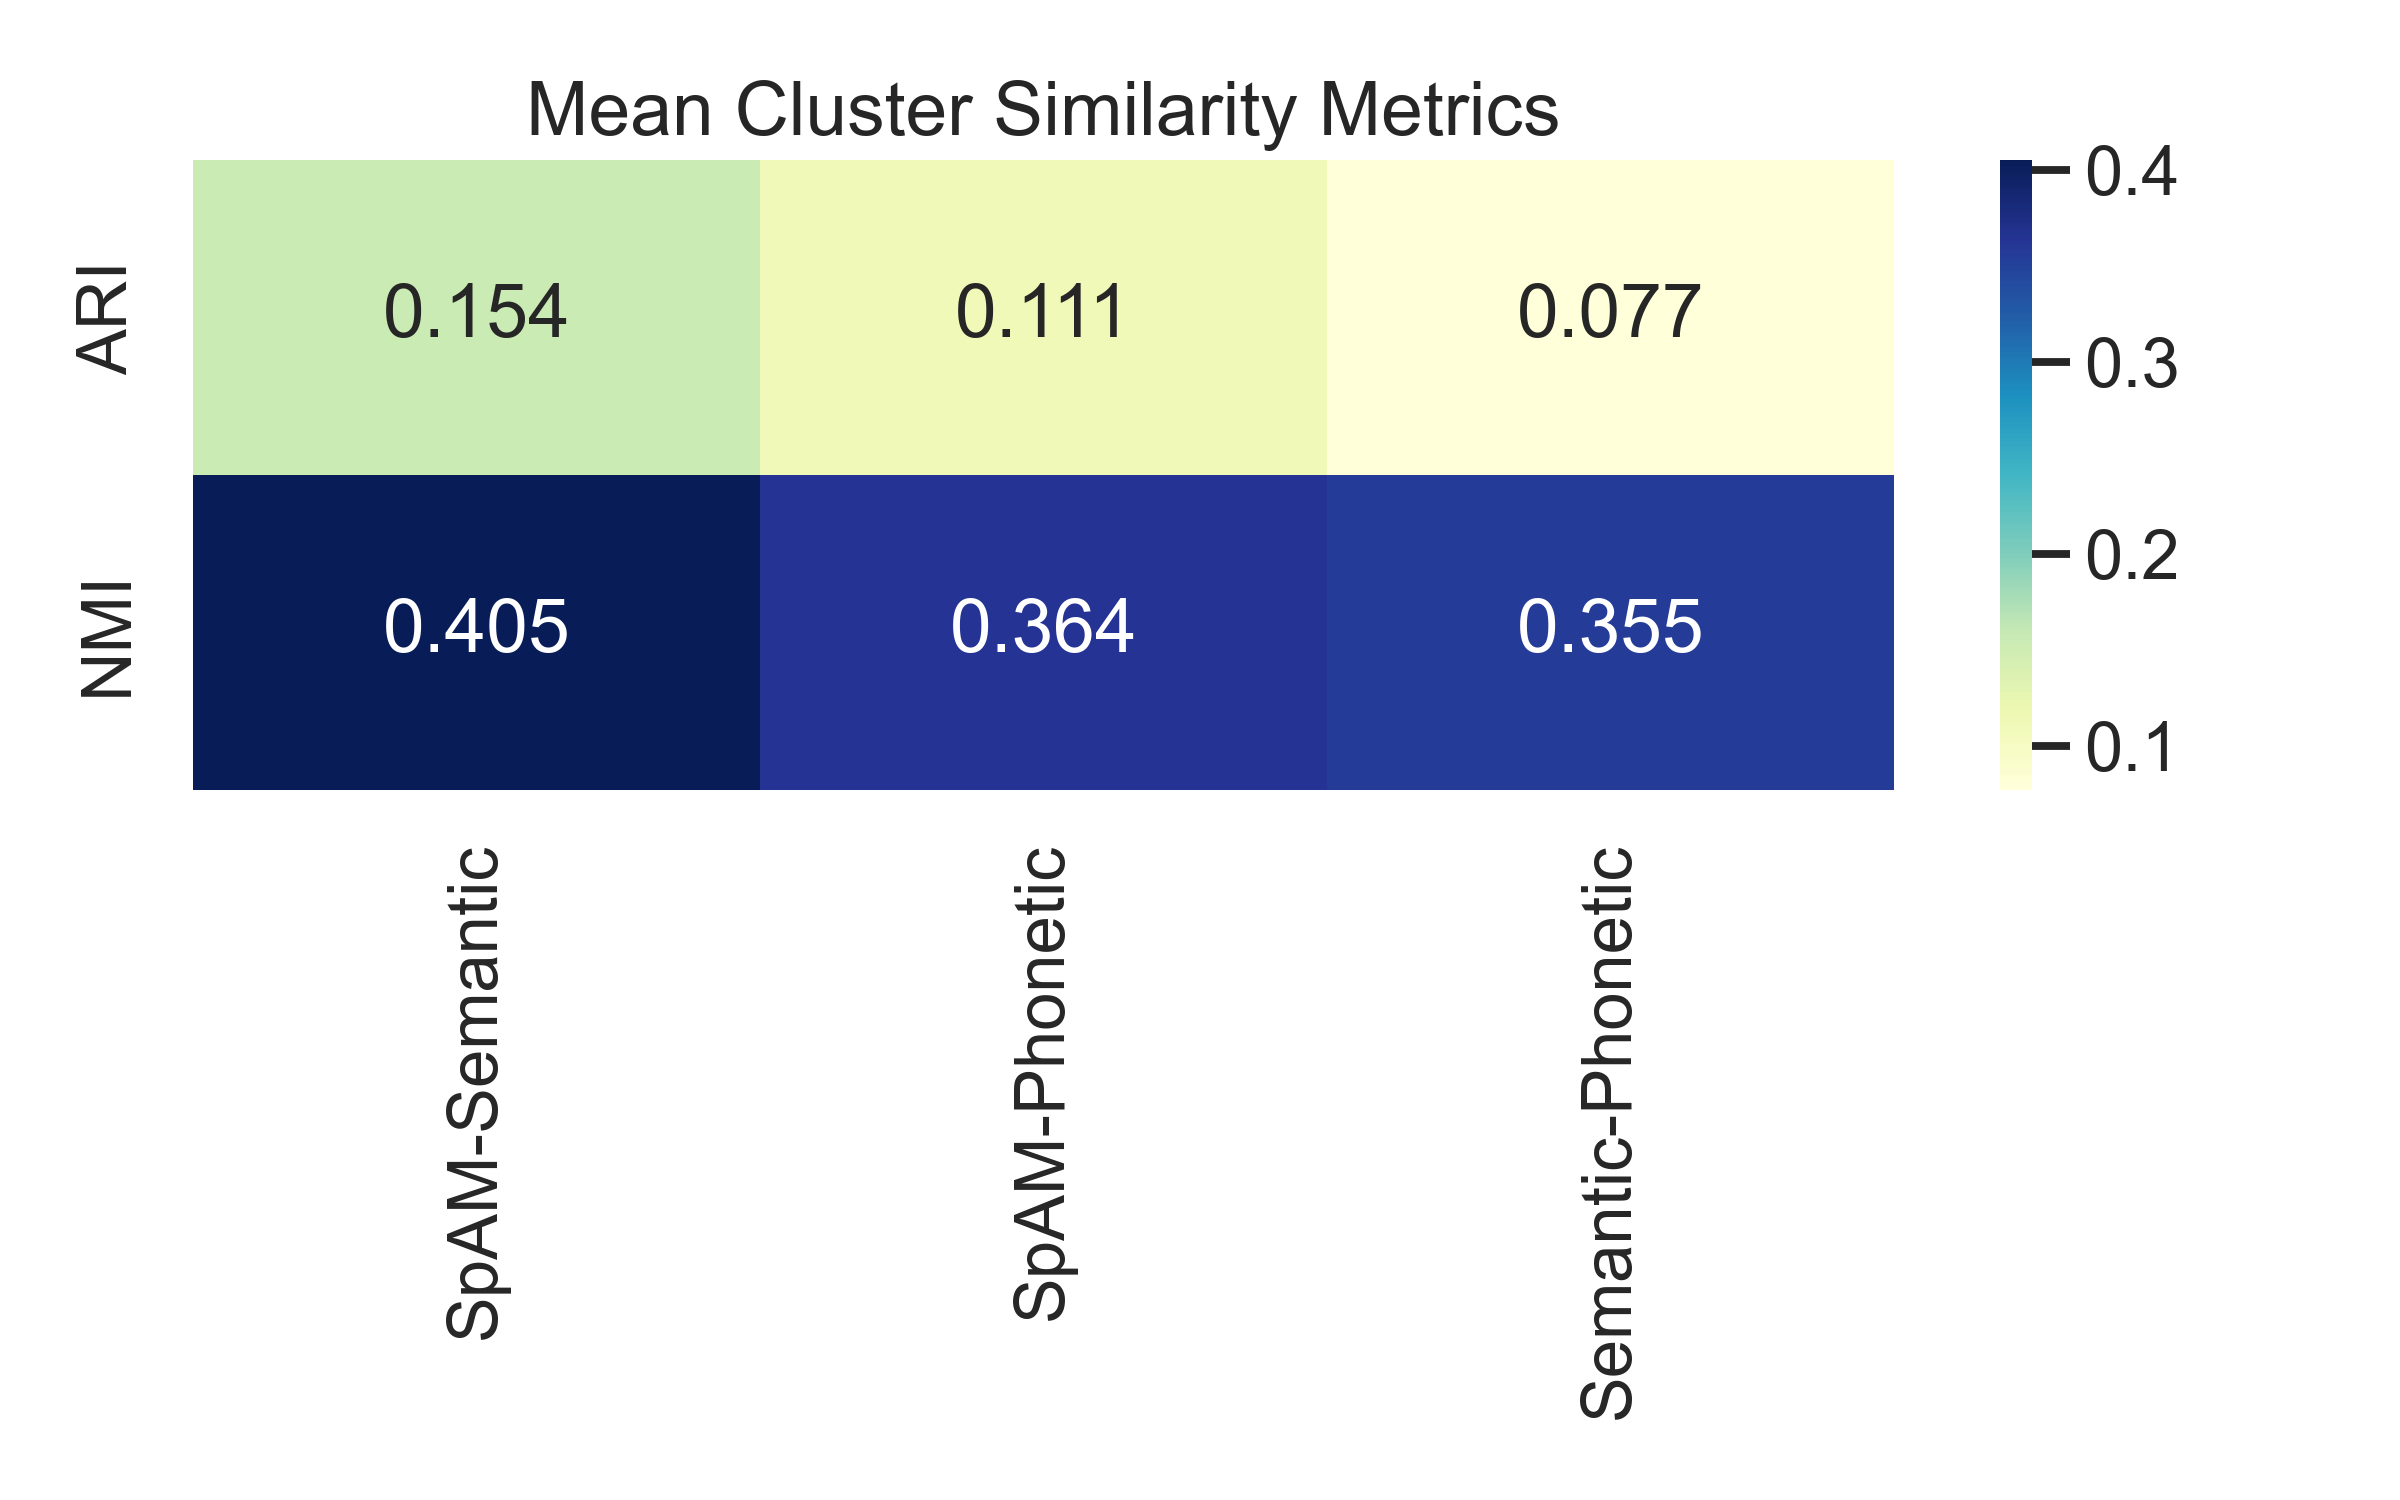
\includegraphics[width=\linewidth]{images/cluster_similarity_matrix.png}
  \caption{Average ARI and NMI values for semantic and phonetic cluster comparisons.}
  \label{fig:sim_matrix}
  \end{figure}

  \begin{figure*}[t]
  \centering
  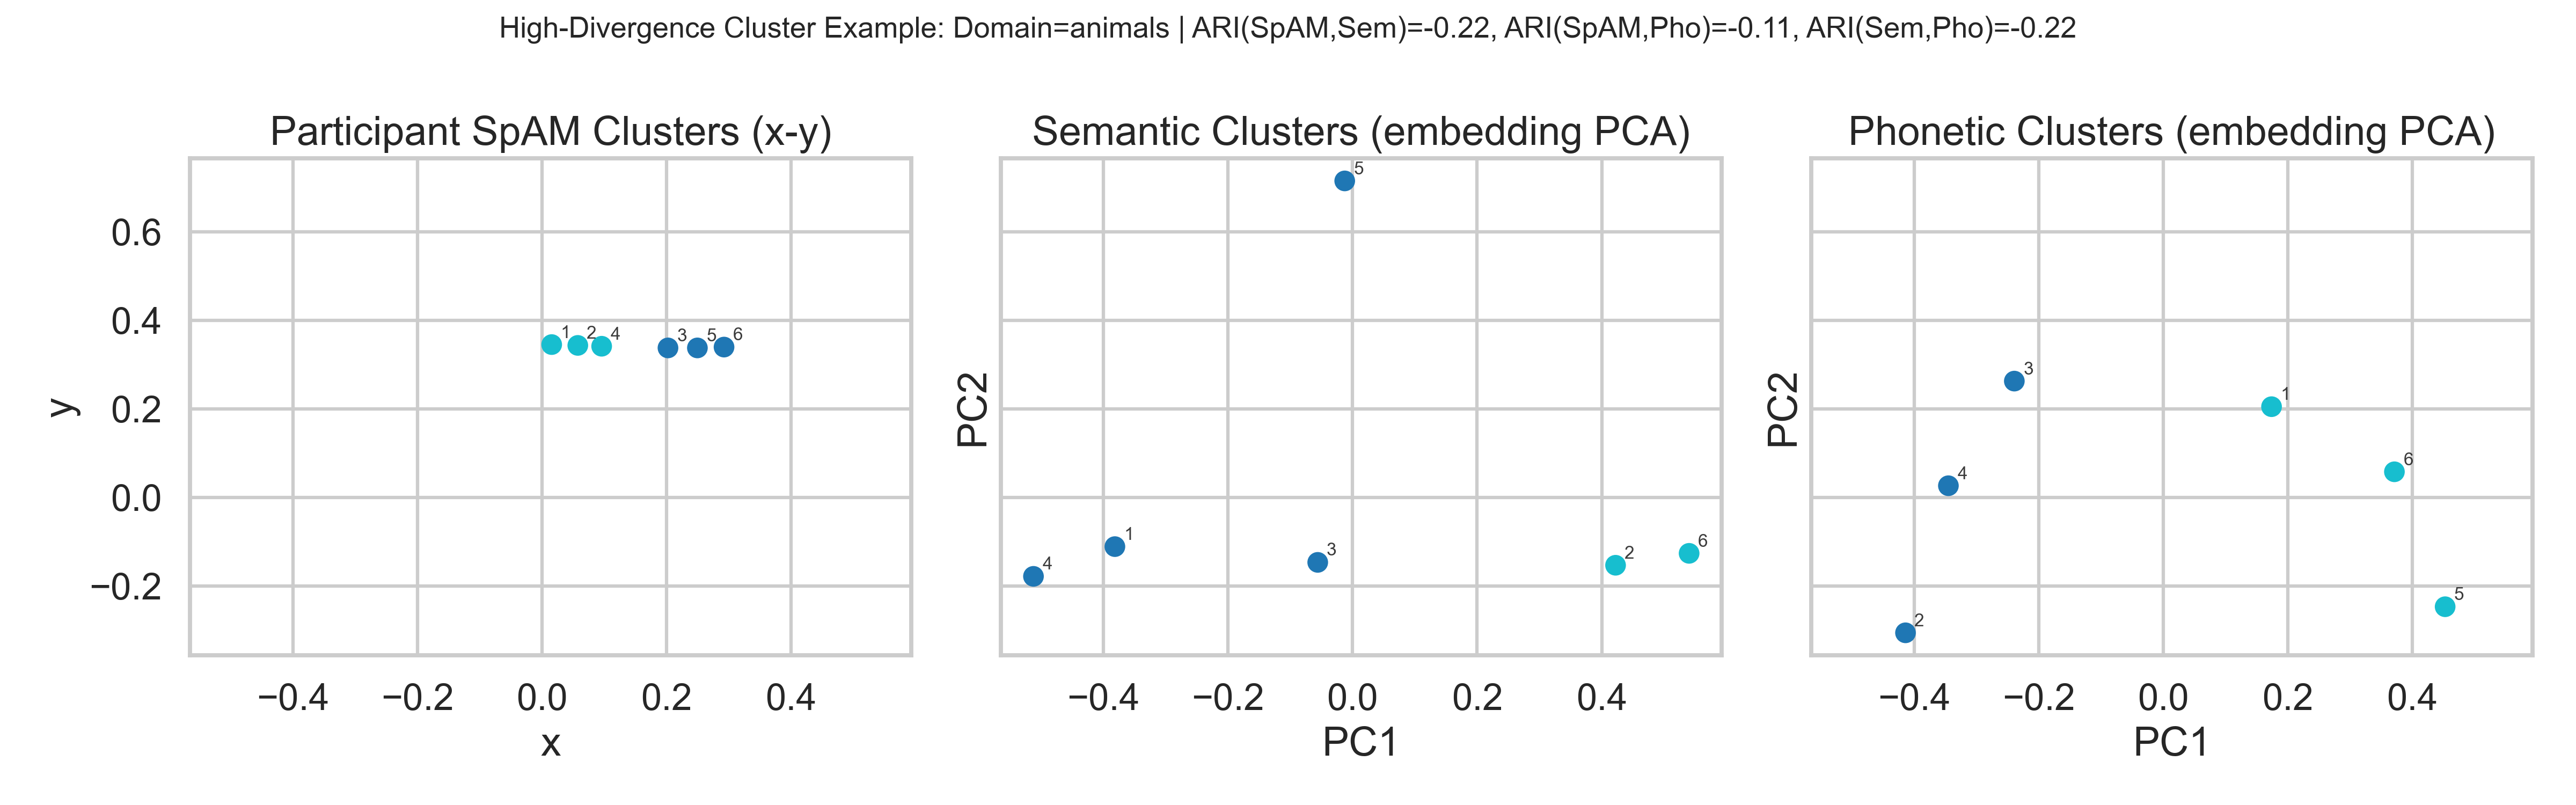
\includegraphics[width=0.94\textwidth]{images/sample_spam_semantic_phonetic_clusters.png}
  \caption{Example participant-domain case: SpAM clusters versus semantic and phonetic cluster assignments.}
  \label{fig:cluster_example}
  \end{figure*}

  \textbf{Inference.}
  For RQ4, sign tests and NMI both support non-trivial positive alignment with semantic and phonetic representations, with stronger average overlap in the semantic channel.

\subsection{Composite Fluency Score}
  \textbf{Question addressed (RQ5):} Does combined VFT+SpAM scoring improve over VFT-only scoring?

The integrated score combines VFT and SpAM features with equal domain weights.

For comparison with self-reported Hindi confidence:
\begin{itemize}
    \item VFT-only score: $\rho=-0.449$, $p=0.0069$.
  \item Integrated score: $\rho=-0.317$, $p=0.0633$.
\end{itemize}

  \begin{figure}[t]
  \centering
  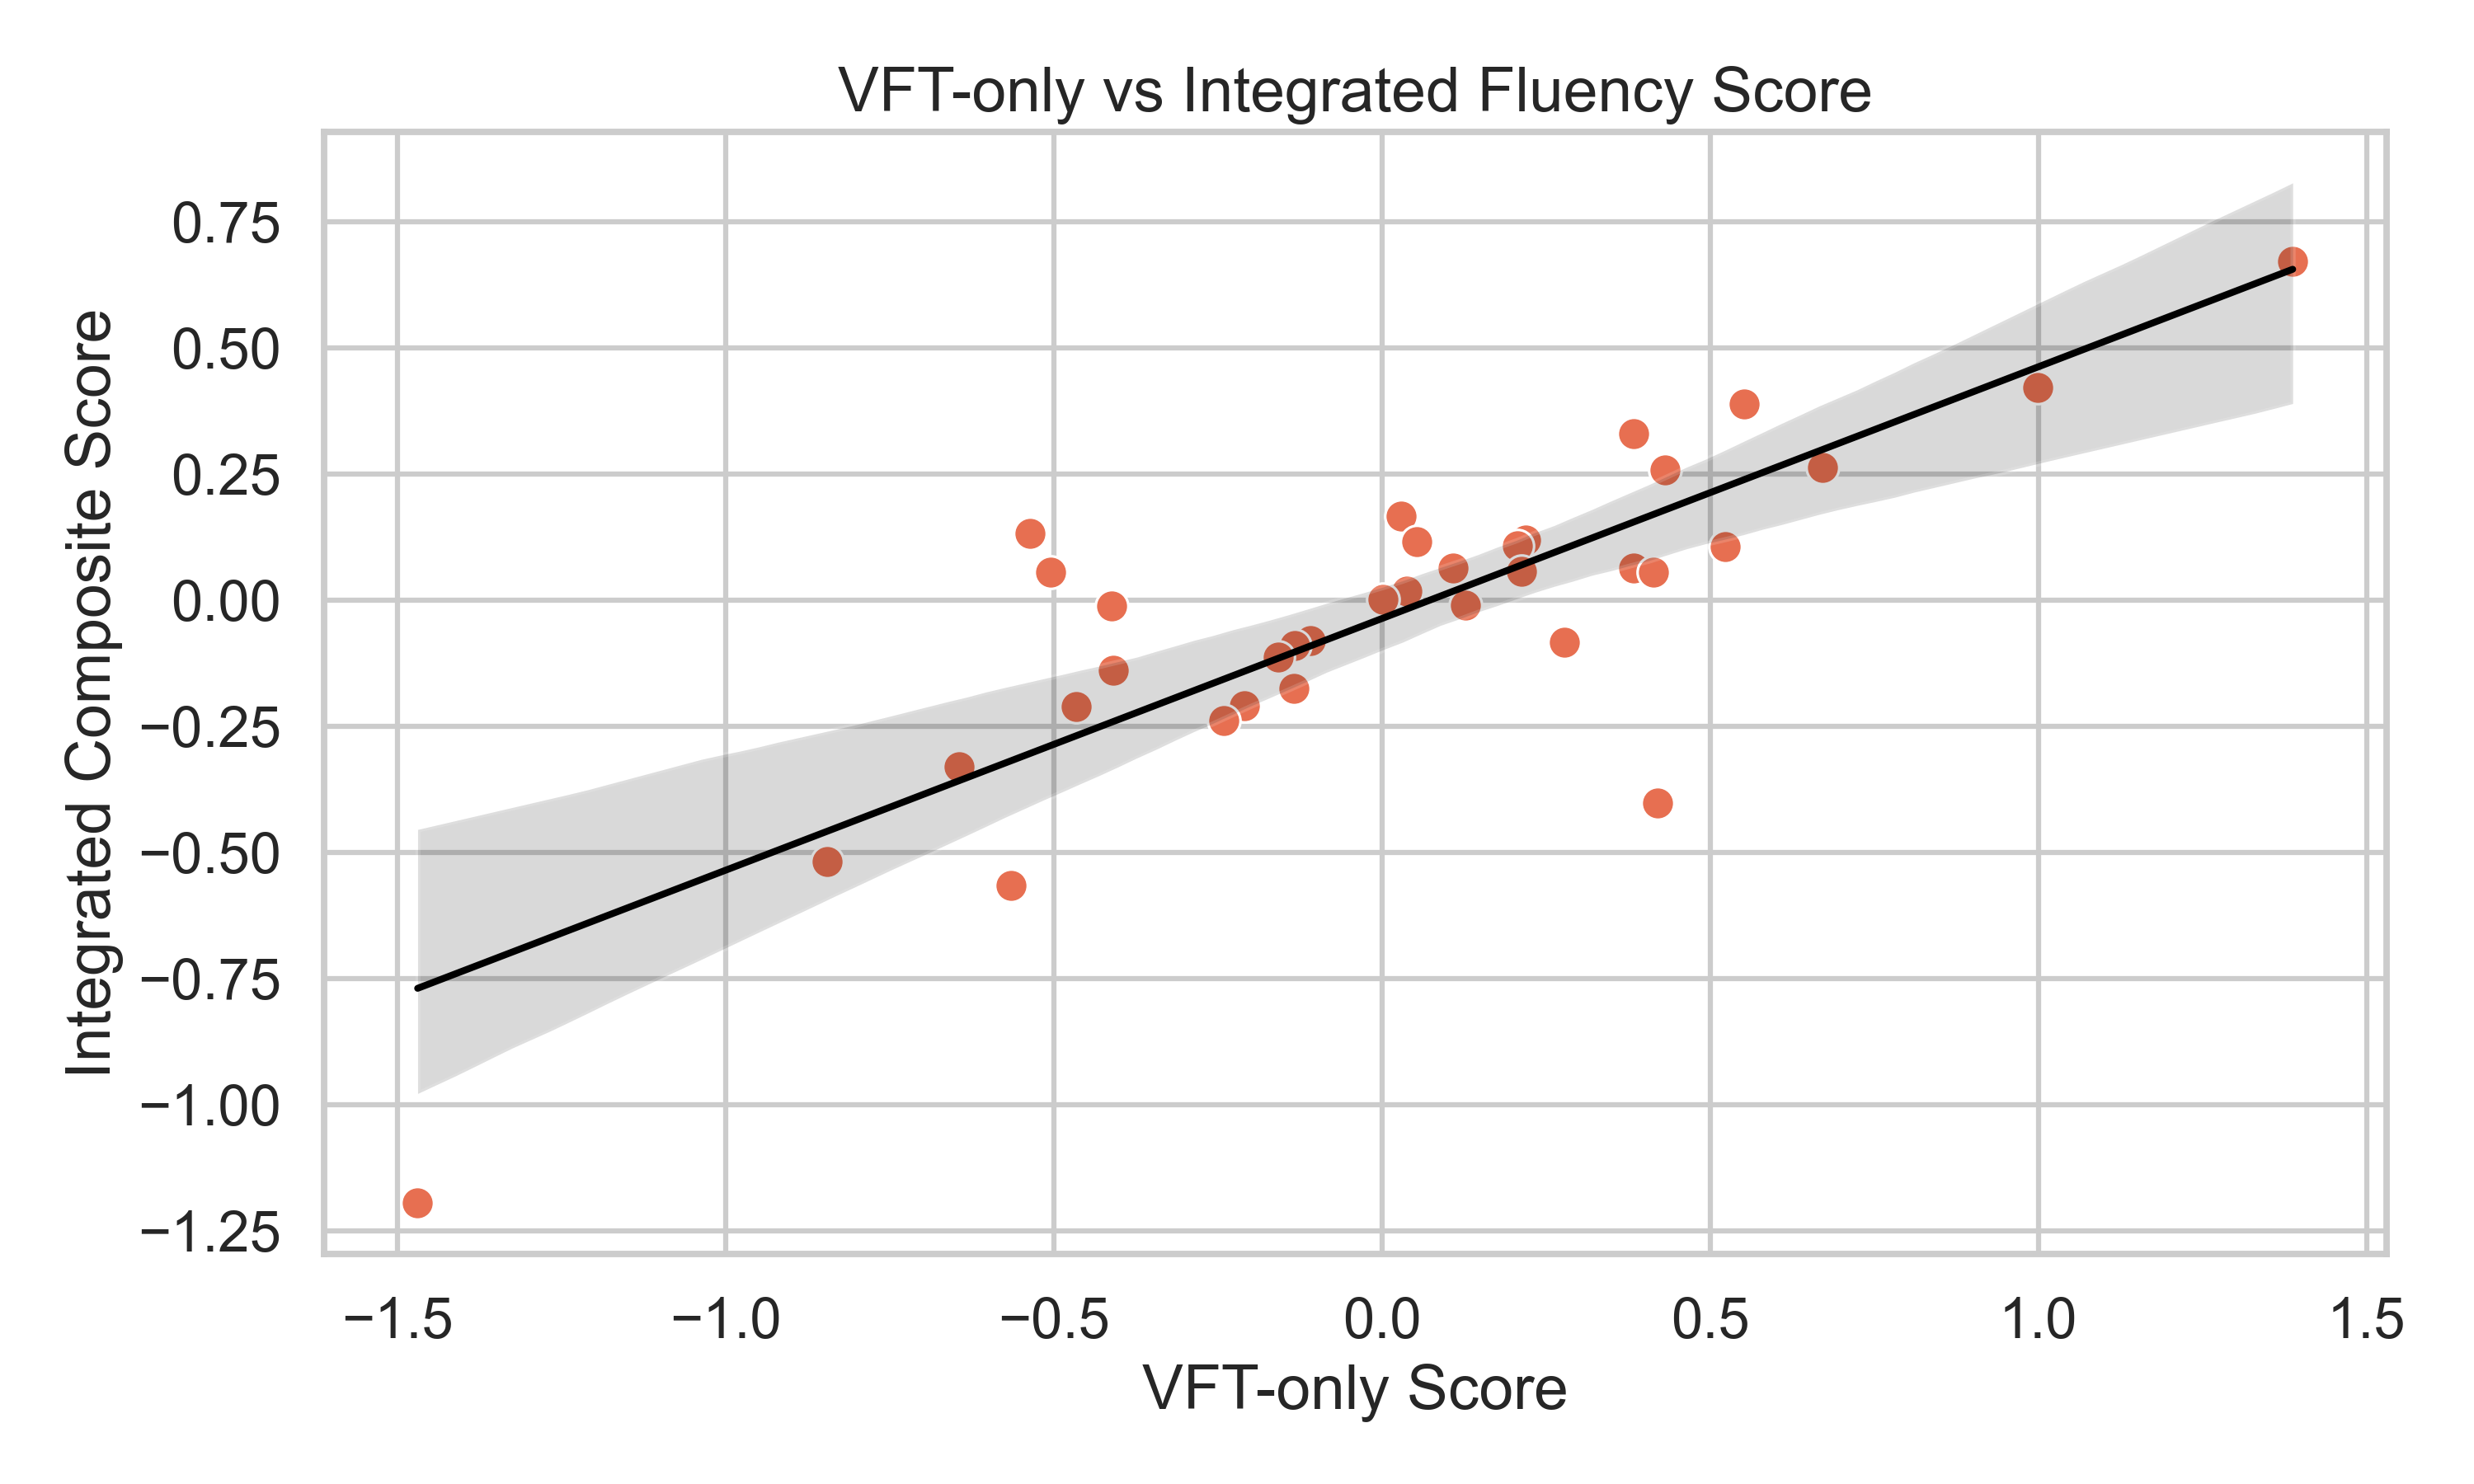
\includegraphics[width=\linewidth]{images/vft_vs_integrated_score.png}
  \caption{VFT-only score versus integrated (VFT+SpAM) composite score.}
  \label{fig:vft_integrated}
  \end{figure}

  \begin{figure}[t]
  \centering
  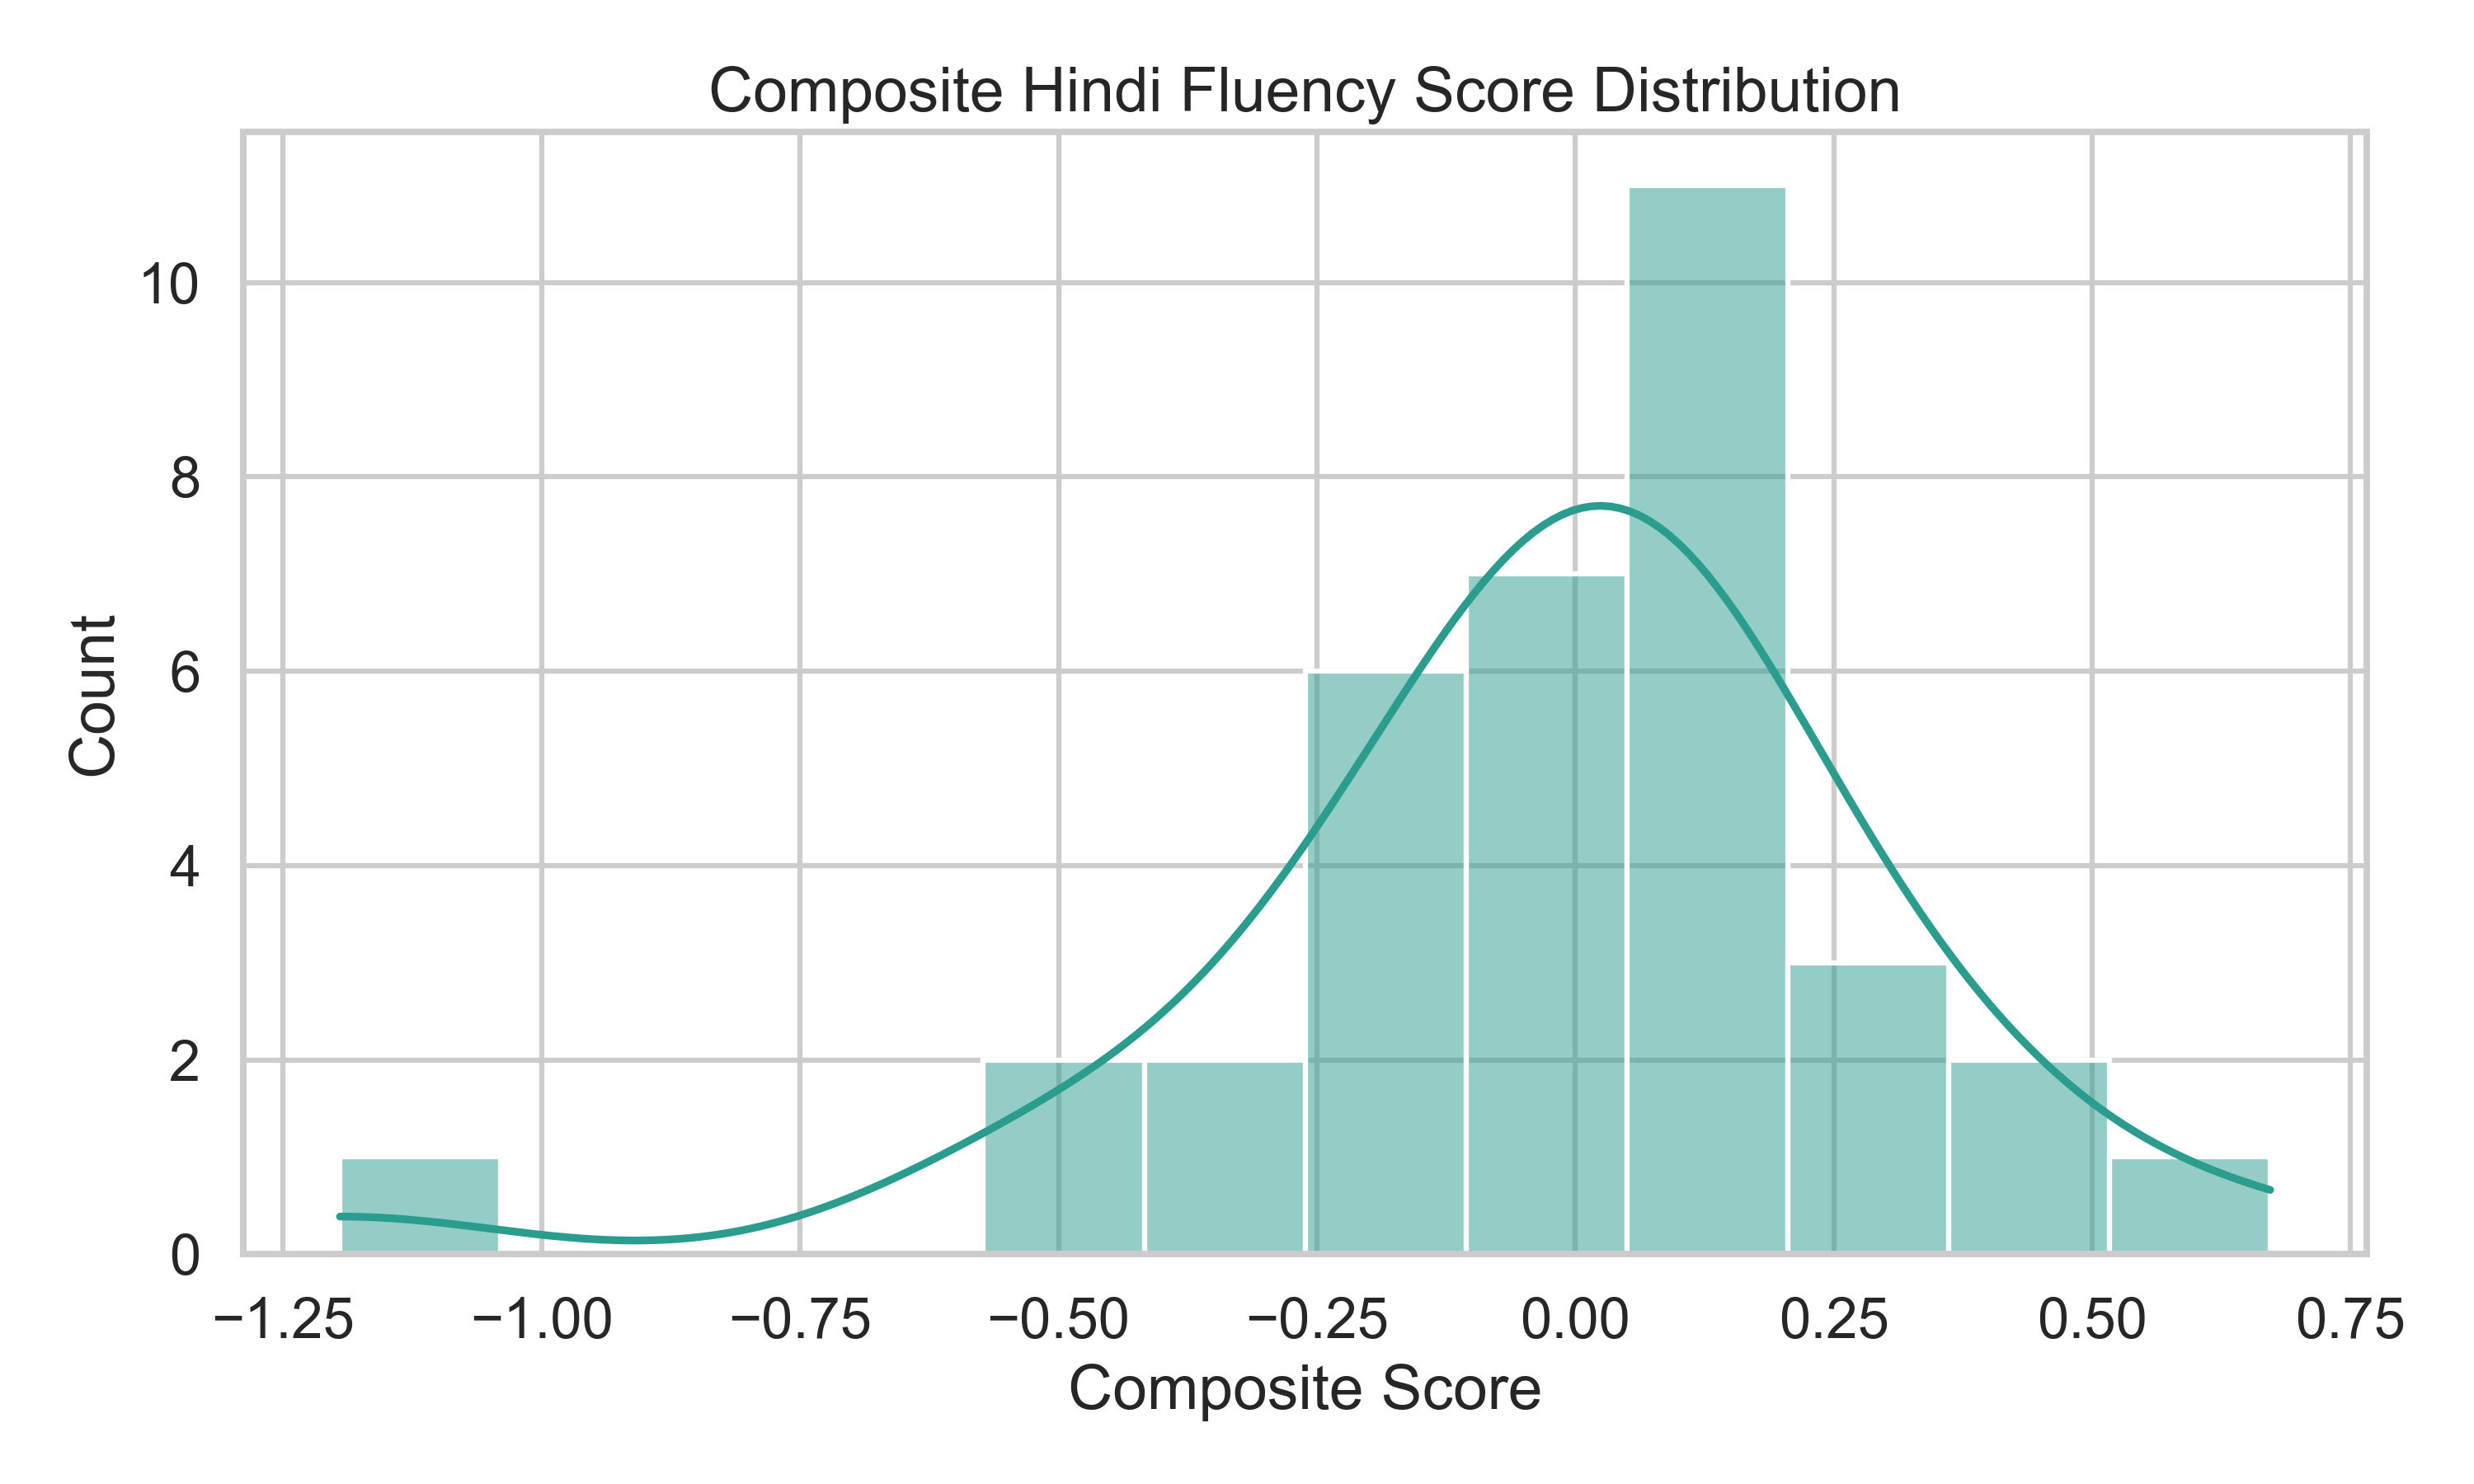
\includegraphics[width=\linewidth]{images/composite_score_distribution.png}
  \caption{Distribution of integrated composite Hindi fluency score.}
  \label{fig:comp_dist}
  \end{figure}

  \textbf{Inference.}
  For RQ5, integrated scoring does not show stronger association with confidence than VFT-only scoring in this dataset and is not significant at $\alpha=0.05$. However, it still adds structure-sensitive information from SpAM and may be useful for broader fluency profiling.

  \subsection{Question-wise Summary}
  Table~\ref{tab:rq_summary} provides direct mapping from each question to statistical outcome and inference.

  \begin{table*}[t]
  \centering
  \caption{Research question, result, and inference summary}
  \label{tab:rq_summary}
  \scriptsize
  \begin{tabular}{@{}p{0.07\textwidth} p{0.30\textwidth} p{0.25\textwidth} p{0.30\textwidth}@{}}
  \toprule
  RQ & Question & Main result & Inference \\
  \midrule
  RQ1 & VFT output/speed by domain & Word count: $p=0.1515$; RT: $p=0.5894$ & No significant domain effect \\
  RQ2 & Participant factors vs VFT outcomes & $\rho_{\text{words,conf}}=-0.395$ ($p=0.019$) & Significant association; direction needs caution \\
  RQ3 & SpAM compactness by domain & Kruskal--Wallis $p=0.3857$ & No significant domain effect \\
  RQ4 & SpAM alignment with semantic/phonetic clusters & ARI sign tests significant; NMI $\approx 0.36$--$0.41$ & Positive directional evidence; moderate overlap \\
  RQ5 & Integrated score vs VFT-only score & $|\rho_{\text{integrated,conf}}| < |\rho_{\text{VFT,conf}}|$, $p_{\text{integrated}}>0.05$ & Structurally richer, not stronger for confidence proxy \\
  S1 & VFT transition dynamics (supplementary) & Switch-rate Kruskal--Wallis: $H=1.909$, $p=0.5916$ & Measurable transitions; effects remain descriptive \\
  \bottomrule
  \end{tabular}
  \normalsize
  \end{table*}

\section{Discussion}
The results suggest a structured lexical search process, but with mixed statistical strength across analyses.

First, domain-wise inferential tests are mostly non-significant. This means we should avoid strong claims about stable domain differences for this sample size.

Second, transition-level VFT analysis shows measurable within-cluster and switch behavior, but no strong domain-level switch-rate effect. This is still informative: lexical search strategy appears heterogeneous across individuals, even when group-level contrasts are weak.

Third, the significant negative association between output size and self-reported confidence should be interpreted cautiously. It likely reflects a gap between perceived and actual performance, together with strategy differences and sampling variability.

Fourth, SpAM and embedding clusters show moderate information overlap (NMI), and sign tests indicate positive ARI tendency in both semantic and phonetic channels. This indicates systematic structure linkage, but also leaves room for participant-specific strategies not captured by one global clustering rule.

Finally, adding SpAM features gives a broader fluency profile, even though it did not increase correlation with confidence in this dataset. In simple words, integrated scoring gives richer structure, but not necessarily stronger external association for every target variable.

\section{Conclusion}
This study combines VFT and SpAM to answer how Hindi speakers search their mental lexicons. The evidence supports a structured search process with participant-level heterogeneity. We find descriptive domain patterns, moderate semantic/phonetic-spatial overlap, and meaningful but mixed cross-task coupling. So, lexical search appears organized, but the organization is not uniform across all participants and all domains.

\section*{Limitations}
\begin{itemize}
    \item Sample size is moderate (35 participants), which limits power for subgroup effects.
    \item Phonetic representation is simplified, and richer phonological modeling can improve precision.
    \item External validation targets are limited in the current dataset.
\end{itemize}

\begin{thebibliography}{99}

\bibitem{Kumar2022}
Kumar, A. A., Lundin, N. B., \& Jones, M. N. (2022).
\textit{Mouse-mole-vole: The inconspicuous benefit of phonology during retrieval from semantic memory}.
PsyArXiv preprint.
\href{https://doi.org/10.31234/osf.io/2bazx}{https://doi.org/10.31234/osf.io/2bazx}

\bibitem{Dautriche2016}
Dautriche, I., Mahowald, K., Gibson, E., \& Piantadosi, S. T. (2016).
Wordform similarity increases with semantic similarity: An analysis of 100 languages.
\textit{Cognitive Science}.
\href{https://doi.org/10.1111/cogs.12453}{https://doi.org/10.1111/cogs.12453}

\bibitem{Hout2013}
Hout, M. C., Goldinger, S. D., \& Ferguson, R. W. (2013).
The versatility of SpAM: A fast, efficient, spatial method of data collection for multidimensional scaling.
\textit{Journal of Experimental Psychology: General, 142}(1), 256--281.
\href{https://doi.org/10.1037/a0028860}{https://doi.org/10.1037/a0028860}

\bibitem{Reimers2019}
Reimers, N., \& Gurevych, I. (2019).
Sentence-BERT: Sentence embeddings using Siamese BERT-networks.
\textit{Proceedings of EMNLP-IJCNLP}.
\href{https://doi.org/10.18653/v1/D19-1410}{https://doi.org/10.18653/v1/D19-1410}

\bibitem{Shapiro1965}
Shapiro, S. S., \& Wilk, M. B. (1965).
An analysis of variance test for normality (complete samples).
\textit{Biometrika, 52}(3/4), 591--611.
\href{https://doi.org/10.2307/2333709}{https://doi.org/10.2307/2333709}

\bibitem{Kruskal1952}
Kruskal, W. H., \& Wallis, W. A. (1952).
Use of ranks in one-criterion variance analysis.
\textit{Journal of the American Statistical Association, 47}(260), 583--621.
\href{https://doi.org/10.2307/2280779}{https://doi.org/10.2307/2280779}

\bibitem{Spearman1904}
Spearman, C. (1904).
The proof and measurement of association between two things.
\textit{The American Journal of Psychology, 15}(1), 72--101.
\href{https://doi.org/10.2307/1412159}{https://doi.org/10.2307/1412159}

\bibitem{Hubert1985}
Hubert, L., \& Arabie, P. (1985).
Comparing partitions.
\textit{Journal of Classification, 2}, 193--218.
\href{https://doi.org/10.1007/BF01908075}{https://doi.org/10.1007/BF01908075}

\bibitem{Rousseeuw1987}
Rousseeuw, P. J. (1987).
Silhouettes: A graphical aid to the interpretation and validation of cluster analysis.
\textit{Journal of Computational and Applied Mathematics, 20}, 53--65.
\href{https://doi.org/10.1016/0377-0427(87)90125-7}{https://doi.org/10.1016/0377-0427(87)90125-7}

\bibitem{Shannon1948}
Shannon, C. E. (1948).
A mathematical theory of communication.
\textit{Bell System Technical Journal, 27}(3), 379--423.
\href{https://doi.org/10.1002/j.1538-7305.1948.tb01338.x}{https://doi.org/10.1002/j.1538-7305.1948.tb01338.x}

\end{thebibliography}

\end{document}
